
\documentclass[12pt,letterpaper]{article}
\usepackage{adjustbox}
\usepackage[margin=1in]{geometry}  %set margin
\usepackage{booktabs}   % for pretty tables
\usepackage{url}  % makes nice looking urls
\usepackage{epstopdf}  % can't remember what this is for
\usepackage{appendix}
\usepackage{amsmath,amssymb}  % I think this is for pretty math? who knows...
\usepackage{amsthm}  % I think this is for pretty math? who knows...
\usepackage{pdflscape} % to put some pages in landscape
\usepackage{placeins} %allows FloatBarrier
\usepackage[pdftex]{graphicx}
%\usepackage{subfig}
\usepackage{setspace}  % package for line spacing 
\onehalfspacing %set line spacing to 1.5

\usepackage{natbib}  % for citation hyperlinks
\usepackage{hyperref}  % for citation hyperlinks
\hypersetup{colorlinks,citecolor=blue}  % set citation hyperlinks blue
\pdfminorversion=6
\usepackage{tikz}
\usepackage[justification=centering]{caption}  % to use captionof to caption table/figure outside of \begin{table}
\usepackage{chngcntr} % to reset counter in appendix for figure/table numbering
\usepackage{subcaption} %to do subtables

\usepackage[utf8]{inputenc} % I don't know overleaf put this here

\usepackage{chngcntr}

\usepackage[parfill]{parskip} % style to have the paper use paragraph skips and no indents.  Feel free to change if you hate it
\usepackage[section]{placeins}
\usepackage{comment}
\usepackage{todonotes}
\usepackage{color}

\usepackage{amsthm}
\newsavebox{\measurebox}
\newtheorem{theorem}{Theorem}
\newtheorem{corollary}{Corollary}[theorem]
\newtheorem{prop}[theorem]{Proposition}

%%%%%%%%%% Store some important variables %%%%%%%%%%

%Re: 12/7 email from AA to DD
\newcommand{\FullNFUSSurveySampleSize}{662}
\newcommand{\PYMKUSSurveySampleSize}{436}
\newcommand{\NFnPYMKIndiaSurveySampleSize}{200}
\newcommand{\ProlificSampleSize}{300}
\newcommand{\RecentInteractionsSampleSize}{104}
\newcommand{\StudyAboutSampleSize}{50}
\newcommand{\NoFurtherSampleSize}{122}
\newcommand{\numposts}{37,347}
\newcommand{\numhposts}{28,752}
\newcommand{\numrecs}{25,593}
\newcommand{\numinteract}{1,050}
\newcommand{\numhinteract}{908}
%%%%%%%%%% Title Page %%%%%%%%%%



\title{\vspace*{-.75in} Algorithmic Curation Creates Bias: Theory, Experiment and Evidence From Facebook\thanks{
For helpful comments we thank Hunt Alcott, Josh Dean, Jonathan Guryan, Reid Hastie, Sam Hirshman, Alex Imas,  Jon Kleinberg, Alex Koch, Devin Pope, Jon Roth, Avner Strulov Shlain, Alex Todorov, Oleg Urminsky, Bernd Wittenbrink, George Wu, attendees at the annual meetings of the American Economic Association and the Society for Judgment and Decision Making, and seminar participants at the University of Chicago. For research support we thank Becky White, Bryan Baird, Amy Boonstra, and the team of RAs at CDR, Tirtha Patel, Pavan Mamidi, and the team of RAs at CSBC at Ashoka University, and the Harvard Decision Science Lab.
}  }

\author{ \vspace*{-.5in}%
\begin{tabular}[t]{cccc}
&  &  &  \\
Amanda Agan &  &  & Diag Davenport \\
\textit{Rutgers University} &  &  & \textit{University of Chicago} \\
\\
Jens Ludwig &  &  & Sendhil Mullainathan\\
\textit{University of Chicago} &  &  & \textit{University of Chicago} \\
&  &  &  \\
%\multicolumn{4}{c}{\textbf{PRELIMINARY AND INCOMPLETE - PLEASE DO NOT CIRCULATE}}  \\
&  &  &  \\
\end{tabular}%
}
\date{\today \vspace*{-0.15in}}


\begin{document}



\maketitle

%%%%%%%%%% Abstract %%%%%%%%%%

\begin{abstract}
\singlespacing
Increasingly we choose from algorithmically-curated choice sets. The options we face, and how they're ranked, are determined by an algorithm that has learned what we like. These algorithms, however, are built on a faulty behavioral premise: in learning what we like, they equate our choices with our preferences. A moment of introspection (and a mountain of research) reveals that this presumption is mistaken. The gap between what we choose and what we actually want is particularly noteworthy in the case of discrimination: many people who abhor prejudice nevertheless implicitly discriminate against "outgroup" members. We show in both theory and experiment how this presumption leads algorithms astray: they end up not just mirroring our biases, but in fact exaggerating them. An empirical audit of Facebook's algorithms across two countries (the US and India) reveals a pattern of bias that is consistent with our model and quantitatively large. We argue these problems are endemic across many applications and requires rethinking how we algorithmically curate choice sets.
\end{abstract}

\newpage

%%%%%%%%%% Begin Actual Paper %%%%%%%%%%

\section{Introduction}



%\todo[inline]{Todo}
%\todo{Todo}
potential intro outline
\begin{enumerate}
    \item Facebook matters. Weak ties and jobs, opinions, exposure reduces discrimination 
    \item Choices are not people's own but mediated by algorithms. These algorithms though are built on a behavioral error: revealed preference.  Model.
    \item We audit these algorithms for bias. PYMK and Newsfeed
    \item Experimental recreation. 
    
\end{enumerate}

\todo[inline]{For sendhil: 1. Need to more precisely differentiate general bias (favor ingroups) form the additional bias that comes from our choices. 2. Link to implicit bias algorithms paper(s). }
Algorithms increasingly must learn our preferences. The set of choices in many contexts have gotten so large that algorithms are needed to help us sift through them and prioritize our attention. For example, algorithms sort Facebook posts and tweets, recommender systems suggest movies to watch, items to purchase and even which candidates an employer might want to consider. So while people do the choosing, algorithms do the curating.  
\todo[inline]{Cite Svirsky paper}
% NEW PARAGRAPH ON WHO CARES ABOUT WHETHER FACEBOOK SHOWS YOU THIS OR THAT POST (TO BE MOVED AROUND AND INTEGRATED INTO INTRODUCTION WHENEVER WE SIT DOWN TO REVISE THE PAPER)
The importance of algorithmic bias with Facebook is suggested by previous studies of the effects of Facebook on social capital, together with research on the effects of social capital on a variety of outcomes of economic and societal consequence. \citep{putnam2000bowling} distinguishes between “bonding” social capital, or “strong ties” with friends and families that provide emotional and other supports, and “bridging” social capital, or “weak ties” \citep{granovetter1973strength}, that provide people with valuable new information and perspectives. The advent of social media has added a third category to this list, “maintained” social capital, or the ability to perpetuate ties to people with whom one has lost face-to-face contact \citep{ellison2007benefits}. Existing research suggests that use of Facebook at all relative to no use, relatively more intensive use of Facebook, and investments in time on “Facebook Relationship Maintenance Behavior” are all associated with increased social capital, particularly the weak ties associated with bridging social capital \citep{antheunis2015impact}. Previous research has found that weak ties are positively related to important outcomes like creativity \citep{baer2010strength}, employment status and income \citep{tassier2006labor}, risk of crime involvement \citep{patacchini2008strength}, health \citep{kawachi2000social}, and subjective well-being \citep{sandstrom2014social}. Previous studies also suggest that intergroup contact over social media, including on Facebook specifically, may reduce prejudice \citep{ALVIDREZ2015533} \citep{schwab2019intergroup}. 


Very often, though, these algorithms learn our preferences only indirectly -- through our choices. The effectively espouse the principle of revealed preference, which even most economists today use only cautiously. After all, a host of research shows that we do not always choose what we want. We are cognitively constrained and might heuristics, have conflicted preferences, and choices can be too easily moved by the context or through social pressure and perceived norms.\footnote{Social scientists across several disciplines including psychology, economics, sociology have documented various scenarios where there exists a gap between preferences and behavior, which can be caused by a myriad of reasons. Terminology can differ between papers---e.g. “experienced utility” and “decision utility”; or “true utility” and “decision utility”; or between “revealed” and “normative preferences” ( \citealt{kahneman1991economic}, \citealt{beshears2008preferences}, \citealt{bernheim2009beyond}). On the use of heuristics see e.g. \citealt{tversky1974judgment}, \citealt{shah2008heuristics}, \citealt{gigerenzer2008heuristics}, \citealt{bordalo2016stereotypes}. On wedges stemming from self-control see \citealt{mischel1989delay}, \citealt{kruglanski2002theory}. On dual-system processing see \citealt{kahneman2011thinking}. On the effect of memory see \citealt{stewart2006decision}. On the effect of attention see \citealt{gabaix2019behavioral}. On the effect of bounded rationality see Simon (1955?) and \citealt{conlisk1996bounded}. On the effect of framing and construal see ([insert construal and framing effects]). On the effect of automaticity see \citealt{dijksterhuis2006making}. On the effect of mistaken beliefs see \citealt{benjamin2019errors} [insert weight and evidence, conservatism, probability weighting from T\&K]. On the effect of social influence see \citealt{asch1951effects}, \citealt{milgram1978obedience}, \citealt{cialdini2004social}. On the effect of culture see \citealt{yamagishi2008preferences} and \citealt{henrich2010beyond}. On the effect of laws and institutions see \citealt{feagin1980discrimination}, \citealt{massey1993american}, \citealt{pager2008sociology}, \citealt{reskin2012race}, \citealt{small2020sociological}, \citealt{north1991institutions}. On the effect of nudges and choice architecture see \citealt{thaler2009nudge}.} 

The wedge between choices and preferences is particularly problematic given concerns about algorithmic bias.\footnote{While this literature is vast, some key studies include \citealt{BarocasHardtNarayan-FairnessBook}, \citealt{BarocasSelbst2016}, \citealt{BolukbasiEtAl(16)}, \citealt{Boyd2012}, \citealt{CaliskanEtAl(17)}, \citealt{Chouldechova2017b}, \citealt{ChouldechovaRoth(20)}, \citealt{CorbettDaviesEtAl2017}, \citealt{CowgillTucker2019}, \citealt{Dwork2012}, \citealt{FusterEtAl(18)}, \citealt{GillisSpiess(19)}, \citealt{HardtPriceSrebro2016}, \citealt{HeidariEtAl(18)}, \citealt{HuChen(18)-WelfareFairness}, \citealt{KamishimaEtAl(11)}, \citealt{KamishimaEtAl(12)}, \citealt{KLMR(18)}, \citealt{KLMS(18)}, \citealt{KLMS(20)-PNAS}, \citealt{KM2019}, \citealt{LiptonEtAl(18)}, \citealt{LiuEtAl(18)}, \citealt{Mayson(18)}, \citealt{MenonWilliamson(18)}, \citealt{MitchellEtAl(19)}, \citealt{ObermeyerEtAl(19)}, \citealt{PleissEtAl(17)}, \citealt{RKM2017}, \citealt{RaghavanEtAl(19)}, \citealt{RambachanEtAl(20)-PP}, \citealt{RambachanEtAl(20)}, \citealt{RambachanRoth(19)-BiasInBiasOut}, \citealt{ZemelEtAl(13)}, and \citealt{ZafarEtAl(19)}. } We know that algorithms can inherit some of our implicit biases such as in language \citep{caliskan2017semantics}. When it comes to choices, psychology suggests that our intergroup biases also show a preference-choice divide. We tend to favor people who belong to the same group as us (e.g. people of the same race, religion, gender, political party, etc.) Such favoritism creeps into our behaviors - and even more so into our less well-thought out behaviors.  Importantly, though, our behaviors reflect {\em greater} favoritism towards the ingroup than we want. 

We build a simple model of how this piece of human psychology interacts with algorithmically constructed choice sets. We show that algorithms trained on data about our behaviors can bake our in-group behavioral bias into the choice sets they they construct for us. The result is that in-groups are doubly favored: the algorithm includes more of the in-group into our choice set; and we continue to favor them in choosing from that set. The in-group is more favored when algorithms aid us in our choices than when we choose on our own. Even people whose behavior is otherwise unbiased themselves can wind up making biased algorithmically-assisted choices because the bias of others leads algorithms to over-represent in-group choices among the set of choices considered. In other contexts, we have seen how algorithms perpetuate our human biases. Here, the combination of algorithmically constructed choice sets and preference-behavior wedges leads to an even more pernicious outcome: algorithms {\em exaggerate} our biases.  

We consider how this mechanism plays out in the context of the largest social media platform in the world: Facebook. Specifically we study two algorithms on the Facebook platform for in-group bias, which we define as over-representation of in-group items in algorithmically-constructed choice sets relative to our own preferences. The main algorithm we study is Newsfeed, a central part of the Facebook experience that takes all the posts of a user's friends then prioritizes them and displays them in ranked order when we log-on. We also study the People You May Know algorithm (PYMK), which helps users construct their social networks by suggesting a list of possible friends from the pool of other users. 

In experiments with US users, we find that Newsfeed ranks own-race posts higher than other-race posts, relative to user's preferences. For example, when we loook at Newsfeed content in the top quartile of subject's explicit preference ranking, in-group posts are about $25\%$ more likely than out-group posts to be among the top five posts shown to users. Out-group posts in the second-to-bottom explicit preference quartile wind up with about the same Newsfeed ranking on average as in-group posts in the very bottom explicit preference quartile. PYMK, on the other hand, shows no in-group preferences. Both these results hold even when we control for other potential confounding factors such as number of mutual friends. 

The differential evidence of in-group bias across the two algorithms is consistent with the psychology of the different types of choices being informed. Algorithmic behavior differs in these two contexts because human behavior differs in these two contexts. The decision about whether to interact with a post happens quickly and frequently - do we dwell on it and read a little longer, click on a comment to expand on it, choose to ``like'' or otherwise react to it, etc. There is not a lot of time spent deliberating. In contrast, we might spend more time on deciding whom to friend, ask ourselves if this is what we want to be doing, a person whose posts we may want to see and whom we want seeing our own musings and pictures. On existing measures of deliberateness, users also perceive these intuitive differences about their own behavior across these two contexts. [ONE NUMBER FROM OUR STUDY?] Newsfeed then is trained on data where there is a bigger gap between preferences and choices; and in fact, it reflects a larger in-group bias. We cannot know for certain all the reasons why these two algorithms differ in their biases. For that, we would need a great deal more access to how they were trained. Still, psychology provides an intuitive explanation. 

%Finally, to assess the generality of these findings, we repeat the experiment in India. Aside from being an interesting context given its sheer scale (1.35 billion people), it also enables us to measure a very different kind of in-group beyond race: religion, specifically Hindus and Muslims. Despite the very different setting and in-group definition, we find almost exactly the same qualitative pattern as before: Newsfeed shows in-group favoritism of a similar magnitude to what we see in the US, and yet again PYMK shows no statistically detectable in-group favoritism. 


\section{A Framework}
People look at a piece of content and then choose whether to engage in it. Engaging in it gives them some utility. They choose so as to maximize utility, but of course implicit biases may shape their choices. Content in our empirical work includes friend's post on Facebook, friend recommendation from Facebook and a movie recommendation in our lab experiment. But the simple framework below applies equally well to someone scanning a tweet and deciding whether to engage with it more closely, X or Y. We denote a piece of content by $s$. 

Each piece of content has features $(x_s)$, such as length of a post. In addition it has a binary feature $g_s$, central to our discussion: $g_s$ equals $1$ if the content was produced by an outgroup member and $0$ if it was created by an ingroup member. Since content is rich  - spanning images and text - the features do not fully characterize it. There is more to $s$ (in driving utility and behavior) than is summarized in $(x_s,g_s)$. Engaging with $s$ produces a real valued $u(s)$. The decision to engage of course depends on utility, but - and this is the key difference from standard models of user behavior - it can deviate from utility. And that deviation can depend on the context of choice. When people are behavior automatically - contexts where they are choosing quickly or mindlessly - they will exhibit more ingroup bias: less likely to engage with posts by outgroup members. We assume the context of choice is a simple binary variable $f=1$ (for fast). Whether a person engages with (or 'clicks') a piece of content is written as $c(s)$  and we assume it obeys: 
$$Pr(c(s) = 1) = \frac{e^{u(s)(1 - b_f g_s)}}{1+e^{e^{u(s)(1 - b_f g_s)}}}$$
Here the extent of user bias is captured by $b_f$: that is the amount by which a post is less likely to be engaged with because it is from outgroup ($g_s = 1$). We assume $b_1 > b_0 \geq 0$ so that the user is implicitly biased and that fast contexts ($f=1$) have greater bias than slow contexts ($f=0$):  Sometimes we will discuss an implicitly unbiased user, by which we mean one who has $b_1 = b_0 =  0$.  Notice that in this model even an implicitly unbiased may still be less likely to engage with outgroup content, 
simply because it gives them greater utility. In this framework - and in the empirical work - we are focusing solely on the additional bias against outgroups, \textit{above and beyond} any preference that might or might not be there in actual utility. Importantly, note that distinction is almost a philosophical one without access to the data on the variation in context: without seeing inconsistent choices across fast and slow contexts, we'd have no way of knowing if a user got greater utility from ingroup posts or if they were exhibiting implicit bias. 

Of course users do not just decide on one post. Instead they face a potentially very large set. We assume there are a set $S$ of $n$ pieces of content. The items in $S$ are chosen iid from a large set of possible content. We assume that the distribution generating $S$ is such that both utility. In particular we assume that 
the distribution of utility satisfies $u(s)\sim N(\beta x,\sigma^2_u)$ and $x\sim N(0,\Sigma_x)$ where $\beta$ is a coefficient vector and $\sigma^2$ and $\Sigma$ characterize the residual variance of utility and the variance-covariance matrix for $x$ respectively.\footnote{Note that we make no particular assumption about $E[u(s)|g_s=1,s\in S] -E[u(s)|g_s=0,s\in S]$: user's actual utility may have a preference for ingroups or not: the extent of that preference plays no role in our analysis.} 


The central problem facing the user - and any algorithm designer - is how to rank this content for the user. Scrolling too all of it is onerous. Absent any algorithm, the content is ranked naturally, such as by the time it was produced. Later, we will model this natural (effectively random) ranking and compare it to algorithmic ranking.  For now we will contrast against benchmarks based on how the user would want the data ranked. Define $r^u(s,S)$ to be a ranking of $S$ according to utility. So the items in $s \in S$ is sorted by $u(s)$ and the highest utility item is assigned rank $1$ and so on. Utility ranking is ideal for the user. 

Of course, utility is unobserved. But choices are observed.  Typically, choices and utility are equated and so ranking by utility is synonymous with ranking by propensity to choose. In practice, therefore, in trying to rank by utility, the goal becomes ranking by choice. Define $r^{c,f}(s,S)$ to be the rank order of content $s$ if S is sorted by $c(s,f)$: the highest consumption item in $S$ will have rank $1$ and so on.  Notice the addition of the $f$ superscript here: how content gets ranked depends on the context of choice. Some content will look more attractive in fast contexts than other content. 

To formalize how ranking by choice - rather than utility - codifies implicit bias, we must we must define our definition of disparity. The \textit{disparity} in any ranking rule $r$ is defined as: 
$$\Delta(r) = Pr(s_0 > s_1 | g_{s_1}= 1, g_{s_0} = 0) - \frac{1}{2}$$ 
That is, draw a random piece of content from the in-group and a random piece of content from the out-group. If these are symmetrically treated, then the odds that in-group content should be rated higher that outgroup content is 1/2. 

With this definition in hand, the first problem of algorithmic ranking becomes clear: algorithms seek to rank by choice, but choice is not utility. Since implicit bias leads to choices that are more discriminatory, the rankings have greater disparities. Specificially, in our setup, it is straightforward to see that: 
$$\Delta(r^u) < \Delta(r^{c,f=0}) < \Delta(r^{c,f=1}) $$
Focusing on engagement increases favoritism for ingroup content; and the disparity rises even further when engagement is measured in fast contexts.

Algorithmic ranking increases disparity, though, above and beyond the problem of using engagement as a proxy for preference. We cannot rank on engagement, but must rank on \textit{predicted} engagement and these predictions create an additional problem. To form predictions, platform must build an algorithm that takes data which involves many pairs of the type $(c,x,g)$ - here are the characteristics of posts and whether the user engaged with it - and from it form an algorithm that predicts engagement for any post using just $(x,g)$. In modeling these algorithms, we will generously assume that the algorithm makes the best possible prediction given an infinite number of data points; specifically for any post the algorithm perfectly predicts $E[c(s,f)|x_s,g_s,f]$.   As a result the algorithmic ranking $r^{a,f}(s,S)$ results from sorting the set of posts by $E[c(s,f) \vert x_s,g_s,f]$. Notice again the importance of $f$: the algorithmic ranking $r^{a,f}$ depends on the $f$ for the context that generated the user data. 

Analogous to the results on choice it is easy to show that algorithms trained on data from fast contexts produce more bias than algorithms trained on data from slow contexts:  $$\Delta(r^{a,f=0}) < \Delta(r^{a,f=1})$$
But they do not simply replicate the bias in engagement. They \textit{magnify} the bias: algorithmic ranking adds an \textit{additional} disparity. In particular, if a user is biased then: 
$$\Delta(r^u) < \Delta(r^{c,f}) < \Delta(r^{a,f})$$ 
The algorithm does not know the actual click rate for every post $c(s)$. Instead it must use the expected click rate, so the average click rate of similar posts, those with the same $(x,g)$. As a result, it is in effect stereotyping the posts: outgroup posts are lumped with other posts; given there is implicit bias, all of them are penalized by being an outgroup post.

The problem can be better seen with  a toy numerical example, much more specific than our normal distribution. Suppose that there are four posts:
\begin{center}

\begin{tabular}{|l|c|c|c|c|}\hline
Post& Group & Utility & Engagement & Algorithmic\\ 
& & & rate & estimate\\\hline 
s&g_s & $u$& $c$ & $E[c|x]$\\\hline 
A & Outgroup & .25 & .2 &.25\\ \hline 
B & Outgroup & .35 &  .3&.25\\ \hline
C & Ingroup & .25 & .25& .3\\ \hline
D & Ingroup & .35 & .35& .3\\ \hline
\end{tabular}
\end{center}
Notice that outgroup posts $B$ and $D$ have the same utility as ingroup posts $A$ and $C$ but are engaged with at lower rates: that is the implicit bias.  The algorithm here has no other $x$ to differentiate posts $A$ and $B$ or $C$ and $D$ so each member of the pair is given the average engagement rate of the pair. This leads to the following ranking:
\begin{center}
    

\begin{tabular}{|l|c|c|c|c|}\hline
Post& Group & Utility & Engagement & Algorithmic\\ 
& &Ranking & Ranking & Ranking\\\hline 
s&g_s&r^{u}&r^{c}&r^{a}\\
A & Outgroup & 4 & 4 &2\\ \hline 
B & Outgroup & 1 &  2&2\\ \hline
C & Ingroup & 4 & 3& 1\\ \hline
D & Ingroup & 1 & 1& 1\\ \hline
\end{tabular}
\end{center}
Ranking by utility would put posts B and D at the top. Engagement favors the ingroup posts: C and D move ahead of A and B respectively. Algorithmic ranking further worsens matters with C now leapfrogging even B. The latter effect happens through a form of stereotyping - C is pooled with other (better) ingroup posts D. 

\subsection{Detectability of bias}

Two other facts are useful to point out - one technical and the other of importance to the world. First, in our setup, standard machine learning algorithms will end up creating ingroup bias \textit{even on data} where there we cannot reject at the $.05$ level the presence of bias. That fact is not in our current setup because by assuming the algorithm can perfectly estimate the conditional expectation function we have abstracted from the fact that data is always finite. When data is finite, however, notice suppose in a sample of $n$ posts, we tried to reject the hypothesis that $H_0: E[c(s)|g_s=0]=E[c(s)|g_s=1]$. A sample may be small enough that we get a p-value of, say, $.2$. The goal of predictive algorithm's however is not to reject hypotheses at the 5\% level. Instead it is to find predictive signal. As such, even in these cases the algorithm will find the signal.  These effects are particularly pernicious if the algorithm finds subgroups (say of $x$) where there is ingroup bias - again not rejectable at the $.05$ level. Then the overall average group difference can be small and yet the algorithm will favor ingroups. 

\subsection{Actual Behavior} 

The second effect involves another phenomena we have not modeled: how users behave when presented with a ranked set of posts.  The reason for ranking is that the set of posts is very large - it is unlikely the user will look through most of it. Intuitively, users will move down the ranked set, looking item by item, and at some point move on.  A (trivial) model of this is that there is some diminishing function $g(r)$ where the user has probability $g(r)$ of persisting until rank $r$. For example if the user has probability $p$ of persisting after each item then $g(r) = p^{r-1}$. A straightforward consequence of users moving on is that later ranked posts are less likely to ever be looked at.  Given a ranked set, therefore, the actual chance of an item $s$ ranked at position $r$ being engaged with is $g(r)c$.  

These two terms $g(r)$ and $c$ suggest two ways that outgroup posts receive less engagement. First, we know that due to implicit bias, wherever the post is ranked the user is less likely to engage with an outgroup post.  Second, though, due to the algorithm outgroup posts are ranked lower. So users are less likely to ever see it. As a result, the algorithm here \textit{exaggerates} the behavioral bias. By ranking posts lower users are less likely to see it and thereby additionally less likely to engage with it. 


%Of course in many cases the platform lacks enough data on any single user so ends up using data on similar users. For any given user $i$ we assume that $L_i$ is the set of users that are "like them". This suggests another ranking rule that might arise. For any For a given user $i$ and any set $S$ we assume $r^{\bar{a},f}(s,S)$ is where $s$ ranks if $S$ is sorted by by $E[c_j(s,f) \vert x_s,f,j \in L_i]$. Thus the platform does not use that user's (expected) click rates to rank but the expected click rates of user's like them. It will be useful to compare these rankings to    Notice that it is important here that for click 

Given these rankings, we are interested in disparities. 





We now consider the algorithm design problem faced by a platform. We assume that the platform has access to some behavioral data. On the basis of this data, it is able to form an algorithmic estimate of $E[c(s)|x_s]$. We will assume in fact that the dataset is sufficiently large that it forms a perfect estimate. So the algorithmic estimate $\hat{c}(s,f) = E[c(s)|x,f]$. 

To understand how this algorithmic estimate may produce "biases", we will first introduce the notion of ranking. Given a set of content $S$, define $r^u(s)$ to be the utility ranking of that content so $r^u(s) = 1$ for the item $s$ with highest utility (with ties broken broken arbitrarily). We can now define the click ranking to be $r^c(s)$ so that 


We assume that user's have preferences over content they want to see. Suppose content $c$ comes from a set of all possible 

Given a piece of content (e.g. a post)  

%%%%%%%%%%%%%%%%%%%%%%%%%%%%%%%%%%%%%%%%%%%%%
%%%%%%%%%%% LAB EXPERIMENT %%%%%%%%%%%%%%%
%%%%%%%%%%%%%%%%%%%%%%%%%%%%%%%%%%%%%%%%%%%%%
\section{Lab Experiment}
We empirically test the implications of our model in two ways. First, we carry out several experiments in the lab (described here) that mimic many of the characteristics of standard online environments where choices are algorithmically curated for users, and show that algorithms exacerbate bias particularly for choices that are least likely to be deliberate and most likely to be automatic, and hence most prone to implicit biases. The advantage of these lab experiments is that because we build the choice-curating algorithm ourselves using study subject data, we know exactly what the algorithm is doing. In the next section below, we repeat the analysis in two field study audits of several real-world Facebook curation algorithms, where we do not have access to how the algorithms are constructed exactly, and show the basic findings from our lab experiments replicate there as well.

\subsection{Study Design}

Our lab experiment mimics the task of an algorithm that must rank that content for the user based on choices from past decisions (potentially of the same user and also other users). Our specific setting involves subjects looking at a series of movie recommendations on a screen, where each movie recommendation is attached to a poster by name (``Amanda A. recommends...'') and choosing amongst a subset of those movies to potentially watch. The movies and posters are shown 3 at a time on the screen, much like results from search algorithms or social media sites might show up. The respondent can click on a button to read a fuller review from the recommender. We selected 45 movies total from a variety of genres; the reviews are taken from the publicly available dataset used in \cite{maas2011learning}.\footnote{Additional informaton about the movies such as pictures to attach to the movies and ratings were taking from \url{IMDB.com}}. 

We use an audit-study design that randomly assigns names to movie reviews, selecting names of the recommenders or posters to signal race and gender saliently from previous studies that have used a similar design to understand different economically-meaningful decisions like hiring (\citealt{BertrandMullainathan(04)}, \citealt{agan2018ban}, \citealt{milkman2012temporal}). The distribution of race among our fictional ``posters'' is designed to mimic the U.S. population overall; in expectation a user would see 64\% white-signalling names, 22\% Hispanic signalling names, and 14\% Black-signalling names. Randomization of names means that we are holding constant the true underlying preference for the movies.

The respondent is instructed to choose 4 movies, and told that once chosen they would get a link to watch one of their chosen movies. Since the recommendations show up 3 at a time, so the respondent needs to click on ``load more'' at least once to choose 4 movies. This is an \textit{incentivized} choice task: subjects were told they would receive one of the four movies they selected for free.

Respondents are randomized into one of two conditions: 
\begin{itemize}
    \item A \textit{rushed} condition in which the subject is told they will have 5 minutes to make their selections, and are told that this is not much time given the task at hand. To reinforce this, the clearly visible countdown clock on the left of the screen counts in milli-seconds so that the numbers are moving quickly while the respondent is deciding.
    \item A \textit{non-rushed} condition in which the respondent is told they have 15 minutes to decide, that this is plenty of time, and the timer counts in minutes, moving much more slowly than in the ``rushed'' condition.
\end{itemize}
Screenshots with instructions and images of both the rushed and nonrushed conditions can be seen in Figure~\ref{fig:lab_images}.

The lab experiment mimics salient features of many online environments in which algorithms help curate people's choices. Users can see limited information about the content, and also see a person attached to that content (Twitter handle/twitter post, Facebook post/name, etc.). Users are able to click to get a little more information before making a decision about whether to engage with the content, which in the case of our lab experiment is to select a movie. The lab experiment also captures the fact that there is variation in the nature of the decisions from which curation algorithms try to learn our preferences, where some of our decisions are made quickly (and hence more vulnerable to implicit bias) while some are made more deliberately.

We recruited study subjects through the Prolific platform. We carried out two versions of the lab experiment:
\begin{itemize}
    \item \textit{Experiment 1} involved $N=981$ study subjects intended to be representative of the US population with respect to race and gender
    \item \textit{Experiment 2} involved $N=753$ study subjects who were white males, a design modification intended to make the job of defining in-group versus out-group posts (one of the key features of our experiment) easier
\end{itemize}
Table~\ref{tab:samplab} shows summary statistics on our subject pools for the first and second lab experiments. The Experiment 1 sample is indeed roughly representative of the country as a whole ($63\%$ white, $23\%$ Hispanic, $14\%$ Black), slightly over-represents females ($61\%$), is more highly educated than the population overall ($32\%$ have a Bachelor's degree and $31\%$ have more than a Bachelor's degree), and has an average age of $29.6$. The study sample for Experiment 2 is somewhat older ($38.8$ years of age) with lower levels of schooling. We have a total of $N=4,859$ movie selections in total for Experiment 1 and $N=3,001$ from Experiment 2. 

The final stage of our experiment involved feeding the results of our two standard lab experiment paradigms into an algorithm-construction pipeline. Specifically, for each study sample separately, we build a machine learning algorithm that takes the subject choices from a given experimental condition (quick decision vs. deliberate decision) within a given lab experiment, then predict's user selections. The output of this algorithm is a rank-ordering of movie choices by the predicted likelihood of user selection. This is basically how actual curation algorithms work, with the only key differences being our dataset is much smaller and we use off-the-shelf machine learning techniques rather than ``industrial-strength'' machine learning.

\section {Lab Experiment Study Results}
Figure~\ref{fig:lab1_click} and Table [DIAG CAN YOU ADD TABLE REFERENCE HERE?] show the main outcomes of  Experiment 1.  When subjects are rushed, they are $3.1$ percentage points more likely to choose a movie recommended by an in-group poster ($p<0.05$; by way of comparison the overall average movie selection rate is XXXX DIAG CAN YOU INSERT?). When subjects are not rushed the in-group selection preference is less than half as large, equal to only $1.4$ percentage points, and is not statistically significant [DIAG CAN YOU CHECK THAT'S TRUE?].   

Figure~\ref{fig:lab1_algo} and Table [DIAG CAN YOU ADD TABLE REFERENCE HERE?] show how the algorithm would sort movie recommendations for subsequent users based on the inputs from our main experiment, separately for subject choices from the rushed and non-rushed conditions.  The vertical axis depicts where each movie gets ranked in terms of number of slots relative to the average movie ranking. In-group posts have a lower ranking (i.e. fall more towards the top of the algorithmic-recommended list) in the rushed state, equal to $2.1$ ranking slots ($p<.05$, equal to XXX percent of the average ranking), while in the non-rushed state in-group recommendations only fall about $1$ ranking slot towards the top, which is not statistically significant (DIAG CAN YOU CONFIRM?) 

The results from Experiment 2 are qualitatively similar as shown in Figure~\ref{fig:lab2} and Table DIAG CAN YOU ADD TABLE REFERENCE HERE?. Figure~\ref{fig:lab2_click} shows that this time around there is suggestive ingroup bias in both conditions, but neither reaches statistical significance. But as the model predicts, when we feed these choices into our algorithm to sort movie recommendations, we see very similar results to lab experiment 1 where there is now a statistically significant up-ranking of in-group posts in the rushed condition ($3.3$ ranking slots, $p<.05$), but again not in the deliberate condition (the interaction between in-group recommendations and the deliberation condition equals $1.4$ ranking slots, $p<.05$).

Recall that standard machine learning algorithms are looking for pockets of signal in the data, not necessarily statistical significance in overall average comparisons. Suppose, for example, that that there are only two genres of movies (horror and everything else), and that in-group bias is only pronounced among horror film selections. Now consider one of the simplest classes of machine learning algorithm, the decision tree. If the first split of the tree is on genre, at the second level of the tree, the algorithm would split by in-group versus out-group status for horror movies but not for other genres. The tree is designed to find this pocket of signal in the data, hence the initial description of algorithms like this in the computer science literature was as ``automatic interaction detectors.'' While the overall average in-group versus out-group differences may not be statistically significant, the in-group versus out-group differences in algorithmic predictions should be more precisely estimated - and so more likely to be statistically significant - because the algorithm's averaging eliminates some of the noise in the actual data.

We have, in sum, just empirically demonstrated with data from actual study subjects that curation algorithms can indeed create a ``double penalty'' for out-group content by learning implicit biases by users. We turn next to the question of whether we see similar patterns in at-scale online curation algorithms out in the real world.

%%%%%%%%%%%%%%%%%%%%%%%%%%%%%%%%%%%%%%%%%%%%%
%%%%%%%%%%% FACEBOOK STUDY %%%%%%%%%%%%%%%
%%%%%%%%%%%%%%%%%%%%%%%%%%%%%%%%%%%%%%%%%%%%%


%%%%%%%%%% STUDY DESIGN %%%%%%%%%%
\section{Facebook Study Design} 

We advertised for study subjects who were Facebook users and were willing to participate in a Zoom-based interview. Study populations were accessed through the University of Chicago Booth School of Business Center for Decision Research (CDR), the Harvard University Decision Science Laboratory (HDSL). Each of these sites maintains a subject pool drawn mainly from the local population.\footnote{CDR recruits participants through posts to Facebook, Twitter, and other social media. HDSL recruits from the local Cambridge community.} Further details on our sample recruitment protocol can be found in Appendix~\ref{app:materials}.

Subjects were first asked to complete a survey asking about their demographic characteristics and basic Facebook usage patterns. Subjects were then asked to log in to their Facebook account and share their screen. Data was collected in several waves, and different subjects had different data collected depending on the wave they participated in:
\begin{itemize}
    \item For all subjects, enumerators captured the Newsfeed algorithmic ranking, $r^a$, and information about each of the first 60 posts in the user's Newsfeed (N$=$\FullNFUSSurveySampleSize{}).
    \item A subset of Newsfeed subjects then participated in a similar data collection about the first 60 friend recommendations from the PYMK algorithm (N$=$\PYMKUSSurveySampleSize{})
    \item A different subset then participated in data collection about their 10 most recent interactions with Newsfeed posts on Facebook (N$=$\RecentInteractionsSampleSize{})
    \item A final subset had no further data collection (N$=$\NoFurtherSampleSize{})
\end{itemize}
Which data collection a subject participated in was determined by the date and location of data collection---a complete description of this wave structure of the data collection is in Appendix~\ref{app:materials}. In our main analysis we will use the full samples available for each result---that is, we present results for Newsfeed for all observations for which we collected Newsfeed data, results for PYMK in the full sample for which we collected PYMK data, and results for interactions with Facebook posts in the full sample for which we collected interaction data. In Appendix~\ref{app:tab_fig} we present Newsfeed results using only the subsample for which we also have PYMK information.

For the US study we define in-group and out-group by whether the user and the Newsfeed poster (or potential friend being recommended) belong to the same race/ethnic group. In the appendix we replicate our results using the same in-group/out-group definition we use for the lab experiment, although given the difference in decision contexts we believe race is the more relevant definition for the US Facebook analysis. To avoid priming study subjects about the topic of race, and because of time constraints on our data collection with each subject, we did not ask subjects themselves to report the race/ethnicity of posters on Newsfeed. Instead we asked our enumerators, who could see the subject's Facebook account through screen sharing, to record their perception of the  race/ethnicity of the posts from people (not companies) in each of the first 60 total posts and first 60 friend recommendations.

To measure the subject's own race/ethnicity, we asked subjects to self-report using the seven race and ethnicity categories from the US Census, where subjects can check as many boxes as they like. We also asked the enumerators to record their perception of the race/ethnicity of the subject before the Facebook data collection began. In Appendix ~\ref{app:tab_fig} Table X, we show that there is overwhelming agreement between the enumerator perception of the subject's race/ethnicity and the subject's self-report (RA's perception matches the subjects self-identification exactly 85\% of the time\footnote{This is under a very strict definition of match, and given that subjects often chose more than one race but RA's rarely did, a looser definition of match gets an even higher concordance rate.}).

We also collect direct measures of utility, measured by explicit preference for Newsfeed posts and by familiarity for PYMK friend recommendations. We asked subjects to report for each of the posts from people amongst the first 60 total posts they see on Newsfeed: “There are more posts than Facebook can possibly show you. How would you rate this post on a scale from 1-7 where 1 means ‘can skip’ and 7 means ‘definitely want to [see]'''. For those that participated in the PYMK data collection, for the first 60 friend recommendations on PYMK they are asked: “How familiar are you with this person on a scale from 1-7?” where 1 is not familiar and 7 is very familiar.'' The enumerators also record ancillary information about the Newsfeed posts such as how long ago it was posted, whether the post is made by person or company, and whether it was to a Facebook group. For PYMK recommendations, enumerators recorded additional information like how many mutual friends that each friend recommendation has with the subject.

For a subset of subjects we also measured not just preferences for posts, but also their recent behavior on Facebook (N$=$ \RecentInteractionsSampleSize). Specifically we recorded the 10 most recent posts on Newsfeed that the user had some \emph{interaction} with (``liking'' or choosing another reaction or commenting), and exactly what action they took. Enumerators then also recorded the perceived race/ethnicity of the poster.\footnote{The algorithm presumably has access to a wider range of behaviors than this, such as how long the user lingered on a post, whether the user clicked to expand on the post text or comments, whether the user watched a video and how much of the video was watched, etc. Given the constraints on our data collection, interacting with posts was the most feasible measure of actual user behavior on the network.} 

Central to our model is the idea that behavioral bias by humans can create algorithmic bias in these types of settings. Previous research suggests behavioral biases are most pronounced when behavior is not guided by deliberate thought.\footnote{See for example \citet{payne2002best}, \citet{lueke2015mindfulness} and the studies reviewed there} To understand whether and how the Newsfeed and PYMK algorithms differ in the degree to which users make considered decisions, we carried out a separate survey on Prolific to measure the amount of cognitive effort, deliberation, and time spent making choices to interact with posts on Newsfeed versus add a friend from ``People you May Know'' (N$=$\ProlificSampleSize). We draw on existing measures in the literature about, for instance, how well the subject could explain their choices, how much ``mental'' effort they say they put into the behavior, whether the decisions are based on gut feelings or careful consideration, and how much time they usually spend (in seconds) making the decision \citep{bargh_1994}. For more details on our specific measures see Appendix~\ref{app:survey}.

Note that subjects were not made aware that this study was about in-group biases or race, and the exact data being recorded by the enumerator was unknown to the subject. For \StudyAboutSampleSize{} subjects, at the end of the survey we asked ``What do you think the purpose of this study is?'' Not one mentioned race, gender, or other indications of in-group biases.\footnote{Similarly, enumerators were not told the purpose of the study, though they were of course aware they were collecting information on race.}

%We also collected an additional wave of data from India (n$=$\NFnPYMKIndiaSurveySampleSize{}), using same-religion as an in-group definition. For more details on this sample and the results see Section X and Appendix~\ref{app:india}.

%%%%%%%%%% RESULTS %%%%%%%%%%

\section{Facebook Results}

\subsection{Summary Statistics on US Study Sample}

Table~\ref{tab:sumstats_p} shows summary statistics on our subject pool for the US subjects for whom we collected Newsfeed information (N=\FullNFUSSurveySampleSize{}), subjects for whom we collected PYMK information (N=\PYMKUSSurveySampleSize{}), and subjects for whom we collected recent Newsfeed interactions (N$=$\RecentInteractionsSampleSize).  Our subjects are on average in the mid-20s (mean$=26.6$, sd$=$9.186, range$=$18 to 69). A large fraction of our sample check Facebook at least weekly. Compared to all US adults, our samples tend to have a higher proportion Asian, female, and people with a four-year (bachelor's) college degree. 
%In the appendix we show that re-weighting the data to demographically match the rest of the US with respect to gender, race and ethnicity yields qualitatively similar findings. (CHECK) 

The preference and familiarity ratings we collected vary substantially between subjects in terms of both the mean rating and the variance of these ratings, which is presumably due to some combination of differences in the distribution of types of posts across subjects and differences across subjects in how they interpret and use the Likert scale. So rather than rely on the raw preference responses, which are hard to compare across subjects, we create within-subject normalized preference rankings to use in our analysis. 
%For completeness we show in the appendix that our main results also hold when we analyze the data using each study subject's actual raw Likert scale rating for each post instead. (THAT'S TRUE RIGHT?)

From these subjects we collected data on a total of \numposts{} Newsfeed posts, of which \numhposts{} were from people (not companies) and thus included in our analysis sample; \numrecs{} PYMK friend recommendations; and a total of \numinteract{} interactions of which \numhinteract{} were interactions with posts from people (not companies).\footnote{Even the total numbers do not add up exactly to \FullNFUSSurveySampleSize{}$\times$60 and \PYMKUSSurveySampleSize{}$\times$60 because we were not always able to capture a full set of 60 for each subjects. For 80\% of subjects were able to collect 60 posts on Newsfeed, amongst those we did not collect the full 60 on average we were able to collect 40. On PYMK we were able to collect the full 60 recommendations for 94\% of the sample.  This could happen due to multiple reasons: although generally one is able to continuously scroll through the Newsfeed for some subjects the algorithm would not show more than X$<$60 posts; because the Newsfeed refreshes each time you go go the home page, if someone accidentally clicked on a post then tried to go back the Newsfeed would refresh and we would stop data collection if more than a few posts had already been collected; sometimes there are internet problems that stop data collection prematurely, or subjects wanted to stop because the collection was taking too long.} Table~\ref{tab:sumstats_o} shows summary statistics for these posts, recommendations, and interactions. About 60\% of posts in Newsfeed are from people of the same race. 58\% of friend recommendations are of people of the same race.

\subsection{Newsfeed}

We start with results for the most widely used algorithm on Facebook, the one each user encounters as soon as they log-in: Newsfeed. It is useful to compare the algorithm's ranking to some natural alternative, $r^n$, such as reverse chronological order---which is how Newsfeed originally ranked posts until October 2009.\footnote{See \url{https://wallaroomedia.com/facebook-newsfeed-algorithm-history/}.} Using the data we collected on how long ago the post was created, we can compare what a reverse chronological ranking of the first 60 posts would have looked like (shown on the x-axis in the `heatmap' presented in Figure~\ref{fig:nftime_hm}) compared to the actual Newsfeed algorithm rankings (as shown on the y-axis of the `heatmap' Figure~\ref{fig:nftime_hm}, with the top-ranked posts at the top). The algorithm does tend to sort the most recent posts closer to the top, as indicated by the concentration of data points in the upper right corner. But the Newsfeed algorithm is also clearly taking other things into consideration and doing \emph{something} beyond this natural reverse-chronological rank ordering, since the data are not all concentrated along the 45 degree line in the heat map.

Figure~\ref{fig:nfpref_hm} shows that the Newsfeed algorithm is to some degree successful at doing what Facebook reports the algorithm aims to do, which is to show users posts that they are most likely to be interested in.\footnote{See \url{https://www.facebook.com/notes/facebook-app/interesting-news-any-time-you-visit/10150286921207131/}.} The y-axis in the figure is the Newsfeed algorithm's rankings of posts, as before, while the x-axis is now where each post falls within the user's self-reported preference distribution (where the posts the study subject is most excited to see are at the right; we report everything in percentiles within the user's self-reported preference distribution). The Newsfeed algorithm does succeed in putting posts that are particularly high up in the user's preference ranking towards the top of the ranking.

To the right of each heatmap, in Figures~\ref{fig:nftime_s} and ~\ref{fig:nfpref_s} we present this data in a slightly different way, showing the flows from chronological or preference quartiles (at left) into quartiles of the algorithmic ranking (at right). In Figure~\ref{fig:nftime_s} we can see that the most recent posts are disproportionately likely to show up at the top of the Newsfeed ranking (41\%), but the other chronological quartiles are distributed fairly evenly across the Newsfeed algorithmic rankings. In Figure~\ref{fig:nfpref_s} we see similarly that posts in the top quartile of the preference rankings are more likely to end up in the top of the Newsfeed algorithmic ranking (32\%). So the algorithm does take chronology into account, and successfully learns something about underlying preferences, but is also taking other factors into account as well.

Figure~\ref{fig:nf_bygroup} shows us a different aspect of the Newsfeed algorithm: It disproportionately puts in-group posts higher in the algorithmic rankings (the heat map at the right) relative to out-group posts (the heat map to the left). This is pronounced enough to be able to see visually in the raw data. Panel~\ref{fig:nf_bygroup_em} gives a better sense of the relevant magnitudes. We sort posts into bins of 10 based on their Newsfeed algorithm ranking, with higher-ranked posts at the top of the y-axis in the figure. For each ranking bin $g$ \in \{1,..., G\}, we report the share of all in-group posts that fall into that ranking bin ($ a_g = \frac{\text{ \# of ingroup posts in group g }}{\text{\# of ingroup posts in group g + \# of ingroup posts not in group g}} $) minus the share of all out-group posts that fall into that ranking bin ($ b_g = \frac{\text{ \# of outgroup posts in group g }}{\text{\# of outgroup posts in group g + \# of outgroup posts not in group g}}$), divided by the share of all out-group posts that fall into that ranking bin, which we term the "excess mass of in-group posts" (that is, $ ExcessMass_g  = \frac{a_g -b_g}{b_g}$). The posts at the top of Newsfeed's rankings are well above base rate in the share that are in-group ($13.1\%$, standard error $0.6\%$), while posts at the bottom have a share in-group well below base rate ($-6.5\%$, standard error $0.6\%$).

A natural question is whether Newsfeed is simply giving users what they want; is the up-ranking of in-group posts simply due to user preferences? No, at least not according to explicit preferences. Figure~\ref{fig:nf_main} shows in a variety of ways that in-group posts are disproportionately concentrated at the top of the Newsfeed algorithm's rankings conditional on user self-reported preferences. Consider first Figure~\ref{fig:nf_line}. The median of each user's 60 posts of course shows up right in the middle at ranking 29. In panel A we show how far above this median does the average in-group versus out-group post show-up for each of the 4 quartiles of user preference ranking. The first thing to note is that the in-group posts always have large ranking boosts above median than outgroup posts. While this is true all along the spectrum of user preferences, it is particularly true in the lowest quartile where the average in-group posts gets a $1.02$ ranking-slot boost above median on average (standard error $0.27$), while the average outgroup post in this quartile gets a ranking decrease of $0.81$ ranking-slot below median on average (standard error $0.32$). Another way to see the magnitude of the race difference is that an in-group post in the bottom quartile of the user preference distribution has a \textit{higher} Newsfeed ranking than an out-group post in the next-higher preference quartile.

Panels B-D show analogous figures, with the Y-axis now instead representing the probability a post shows up in the top-5, top-15 or top 15. Regardless of how we measure the ranking boost, in-group posts are consistently ranked higher than out-group posts conditional on user self-reported preferences.

Figure~\ref{fig:nf_rankingboost} to the right shows this in a different way. The x-axis again is posts grouped by user preference quartile. For each post we calculate the difference between it's actual Newsfeed ranking and where the post would fall if ranked in reverse chronological order, then show the average of that for each preference quartile on the y-axis, separately for in-group and out-group posts. For the posts that users are least interested in (preference quartile 1), in-group posts show up about 2 slots higher in the Newsfeed actual ranking than are out-group posts. For the highest-ranked posts (quartile 4) the in-group versus out-group gap relative to chronological ranking is about one slot higher for in-group posts. Put differently the in-group posts that subjects report the least interest in (quartile 1) have about the same average rank-ordering by the Newsfeed algorithm as out-group posts in the next-higher user-preference quartile 2.

Interestingly, normalized self-reported preferences about posts do not reveal signs of much in-group bias. Table~\ref{tab:sumstats_o} shows that differences in quartile rankings of normalized preferences between in-group and out-group posts are very similar, and none of the differences are significant at the 5\% level. In Appendix Figure~\ref{fig:prefcdf} we also show a cdf of the normalized preference which lie basically on top of each other.\footnote{Appendix Table X or Figure Y shows there is a difference in raw likert scale rankings by in-group versus outgroup, however this reflects that fact that Black subjects tended to have more in-group friends and be more likely to use likert pref rankings 5, 6, and 7. The normalized preferences take into account within subject differences in the use of the likert scale.} 

\subsection{PYMK}

Figure~\ref{fig:pymk} mirrors Figure~\ref{fig:nf} but for the PYMK algorithm. Here we consider the natural ranking, $r^n$, to be the number of mutual friends the subject has with the recommended friend divided by the number of total friends the subject as---that is what percent of the subjects Facebook friend do they have in common with the recommendation. As shown in Figures~\ref{fig:pymkfriend_hm} and Figures~\ref{fig:pymkfriend_s} the algorithm is up-ranking people with whom subjects have relatively more mutual friends in common with. The PYMK algorithm is similarly picking up on user's self-reported familiarity with the potential friend as Figures~\ref{fig:pymkpref_hm} and Figures~\ref{fig:pymkpref_s} show, as those that users report being more familiar with are also more likely to show up higher on the recommendation list. As with Newsfeed, the PYMK algorithm is partly reflective of what seems like a reasonable natural ranking (friends in common), and is partly reflective of user's self-reported preferences (the degree to which subjects know the people being recommended), though clearly other factors are at play as well with the algorithm.

In contrast to the Newsfeed algorithm, however, we see little evidence of in-group bias in the PYMK algorithm. The heat maps in Figure~\ref{fig:pymk_bygroup_hm} show how recommendations are ranked by the PYMK algorithm separately for in-group and out-group recommendations. Unlike with Newsfeed, there is little visual difference in rankings by in-group versus out-group status. Figure~\ref{fig:pymk_bygroup_em} to the right shows this a different way, where we rank PYMK recommendations by the algorithm's ordering, put them into groups of 10 (y-axis) and show the excess mass of in-group recommendations. The highest-ranked recommendations if anything have negative excess in-group mass (the share in-group is below base rate), and more generally there is no consistent relationship between PYMK ranking and in-group share.

Figure~\ref{fig:pymk_line} shows the similar results as Figure~\ref{fig:nf_line}: how many slots average does a friend recommendation move above the median by familiarity quartile and in-group versus out-group in Panel A and the probability of being in the top 5, 10, or 15 recommendations in B-D. Here we see that the in-group and out-group lines lie nearly on top of each other with no real difference in how the algorithm ranks in-group or out-group recommendations conditional on familiarity quartile. And Figure~\ref{fig:pymk_rankingboost} similarly shows that while potential friends you are more familiar with tend to get a higher average boost in ranking, these is little difference in the mean ranking boost that posts get above the median ranking by in-group and out-group. 

\subsection{Explaining the Difference}
Why do we see evidence of out-group bias with the Newsfeed algorithm but not with PYMK? Our model suggests one hypothesis: Algorithms rely more on user behavior than user preferences, and we are more likely to see a behavior-preference difference towards more in-group bias in cases where the behavior is relatively less deliberate. We expect user behavior with Newsfeed posts, which is compared to PYMK friend recommendations more frequent and lower-stakes, to be less deliberate than user behavior to accept PYMK friend recommendations. 

Figure~\ref{fig:auto_effsize} shows that for each of the nine measures of how deliberate people's interactions are with either the Newsfeed or PYMK algorithm, users report higher levels of deliberation with PYMK than Newsfeed. In this figure we take the difference between the measure of deliberation in interacting with PYMK and that of interacting with Newsfeed, then divide by the pooled standard deviation of the measure (so units are reported in terms of Cohen's d on the y-axis). The advantage in favor of PYMK in terms of how deliberate the behavior is range from about 0.05 standard deviations (for inattention) to around 0.5 standard deviations (carefulness). When we do a principal components analysis across the measures and compare the first principal components, the PYMK advantage over Newsfeed in terms of being more deliberate equal to around 0.4 standard deviations. A simple composite index of the standardized measures suggest a PYMK deliberation advantage of just over 0.2 standard deviations. Figure~\ref{fig:auto_binaries} shows the result in natural units for the two binary measures, while Figure~\ref{fig:auto_likerts} shows the results in natural units for 7 questions asked on a 7-point likert scale measure as well as the simple average composite score. And Figure~\ref{fig:auto_cdf} shows the CDF for responses to the one continuous measure, time it takes the study subject to make a decision (in seconds).

In sum, study subjects report spending more time and make decisions more deliberately for choosing friends on PYMK relative to interacting with Newsfeed posts. This is consistent with our hypothesis that the behavioral wedge (relative to preferences) in the direction of in-group bias should be smaller for PYMK than Newsfeed.

\subsection{Interactions and Behavior}
Our model not only gives us a way to understand the source of algorithmic bias, but also yields a prediction about the magnitude of the consequences. In our model the biased algorithm compounds the user's own bias (or bias of users like her) by showing the user a choice set that over-represents in-group items. So the magnitude of the bias in user's \emph{behavior} at the end of the day should be even larger than the bias we see in the algorithm rankings, given that they choosing amongst this already biased set. 

To explore this hypothesis we collected data on the last 10 \emph{interactions} people had with Newsfeed posts: reactions and comments. This is not a perfect measure of user behavior with Newsfeed, since there are other behavioral dimensions that we cannot mention in our setting (like the time the user had spent looking at each post, which we cannot capture in our lab setting). We present results here just for the sub-sample of respondents for which we have this behavioral measure.

Figure~\ref{fig:behavior} shows that the share of Newsfeed posts that the user has interacted with that are in-group is indeed larger than the share of posts that are in-group among those that the algorithm ranks towards the top of the user's Newsfeed. The confidence intervals here are somewhat large but the excess share of in-group posts among those the user interacts with (user behavior) is between 50\% and 100\% higher than the posts the algorithm puts in the user's top 5, 10 or 15 of the Newsfeed ranking. The algorithm is not merely reflecting our own behavioral biases back to us, it is amplifying those biases in our behavior.

\subsection{Replication Results from India}

Part of what makes Facebook an interesting test-case for our theory is its massive scope. Billions of people around the world regularly use Facebook and rely on its algorithms. To show that our results are quite general, and not specific either to the US context or to defining out-group bias along the lines of race specifically, we replicated our analysis to test for bias in another massive Facebook market: India.

Specifically, we recruited $N=200$ study subjects via the Ashoka University Centre for Social and Behaviour Change (CSBC). In this sample in-group/out-group is defined not by race (which is signaled by user images in the US Facebook context) but rather by religion (signaled by name in the Indian Facebook context). Other than that detail, the study proceeded identically as in the US. In Table DIAG CAN YOU ADD TABLE NAME HERE, we see that for the Newsfeed algorithm in-group posts (defined by religion) are ranked $1.1$ slots higher (towards the top) than are out-group posts ($p<.05$). In contrast, for the PYMK algorithm in-group posts are less than one-fifth of a slot more highly-ranked, a difference that is not statistically significantly different from out-group posts. In Figure XXXX we show the results visually. (Additional results for this India sample are presented in the Appendix.)

The tendency of algorithms to learn our preferences from our worst selves - our implicit biases that our conscious selves reject - to then create a double penalty that further disadvantages out-group members does not appear to be specific to any particular type of bias (race versus religion versus other salient in-group vs. out-group distinctions), or to any particular setting or country context.

%%%%%%%%%% CONCLUSION (OR DISCUSSION) %%%%%%%%%%
\section{Conclusion}
We have seen how algorithms can magnify our biases. They are problematic in another way. When people recognize a gap between their preferences and their choices, they can do something about it. They can adjust their environments and how they approach the choice to bring these two in line with each other. But the algorithm blindly learns from behavior without access to preferences. Since it, not us, constructs the choice set, it impedes the opportunity for us to learn the problem, which can make the gap more persistent.

\pagebreak
\clearpage
\singlespacing 
\bibliographystyle{chicago}
\bibliography{references}

\clearpage
\pagebreak
%%%%%%%%%% TABLES AND FIGURES %%%%%%%%%%

%%%%%%%%%%
%%% LAB EXPERIMENTS: What did it look like?
%%%%%%%%%%

\begin{figure}[ht]
\caption{Lab Experiment Screenshots}
\label{fig:lab_images}
    \begin{subfigure}{1\textwidth} 
        \centering
        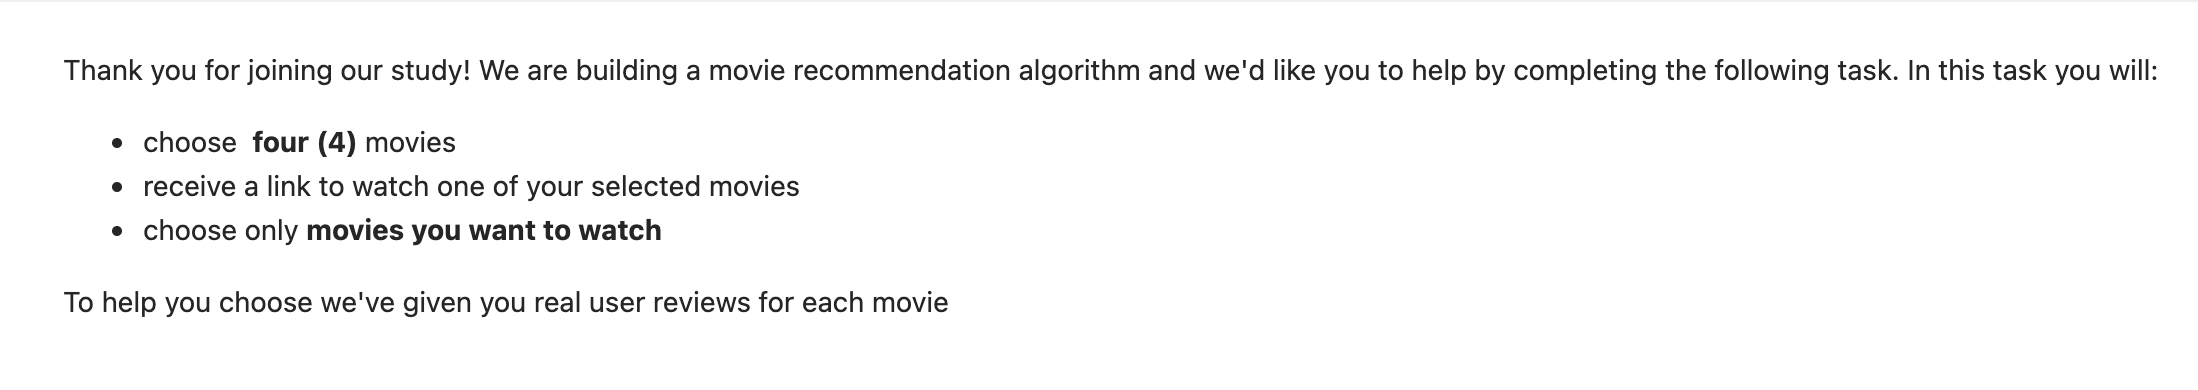
\includegraphics[width=1\linewidth]{Misc Screenshots/LabExpInstructions.png}   
        \caption{Instructions}
        \label{fig:lab_instructions}
        \end{subfigure}
    \begin{subfigure}{.5\textwidth}
       \centering
        
\includegraphics[width=1\linewidth]{Misc Screenshots/NonRushedTimeInstructions.png}  
        \caption{Nonrushed Time Instructions}
         \label{fig:lab_nonrush_instructions}
    \end{subfigure}
     \begin{subfigure}{.5\textwidth}
       \centering
        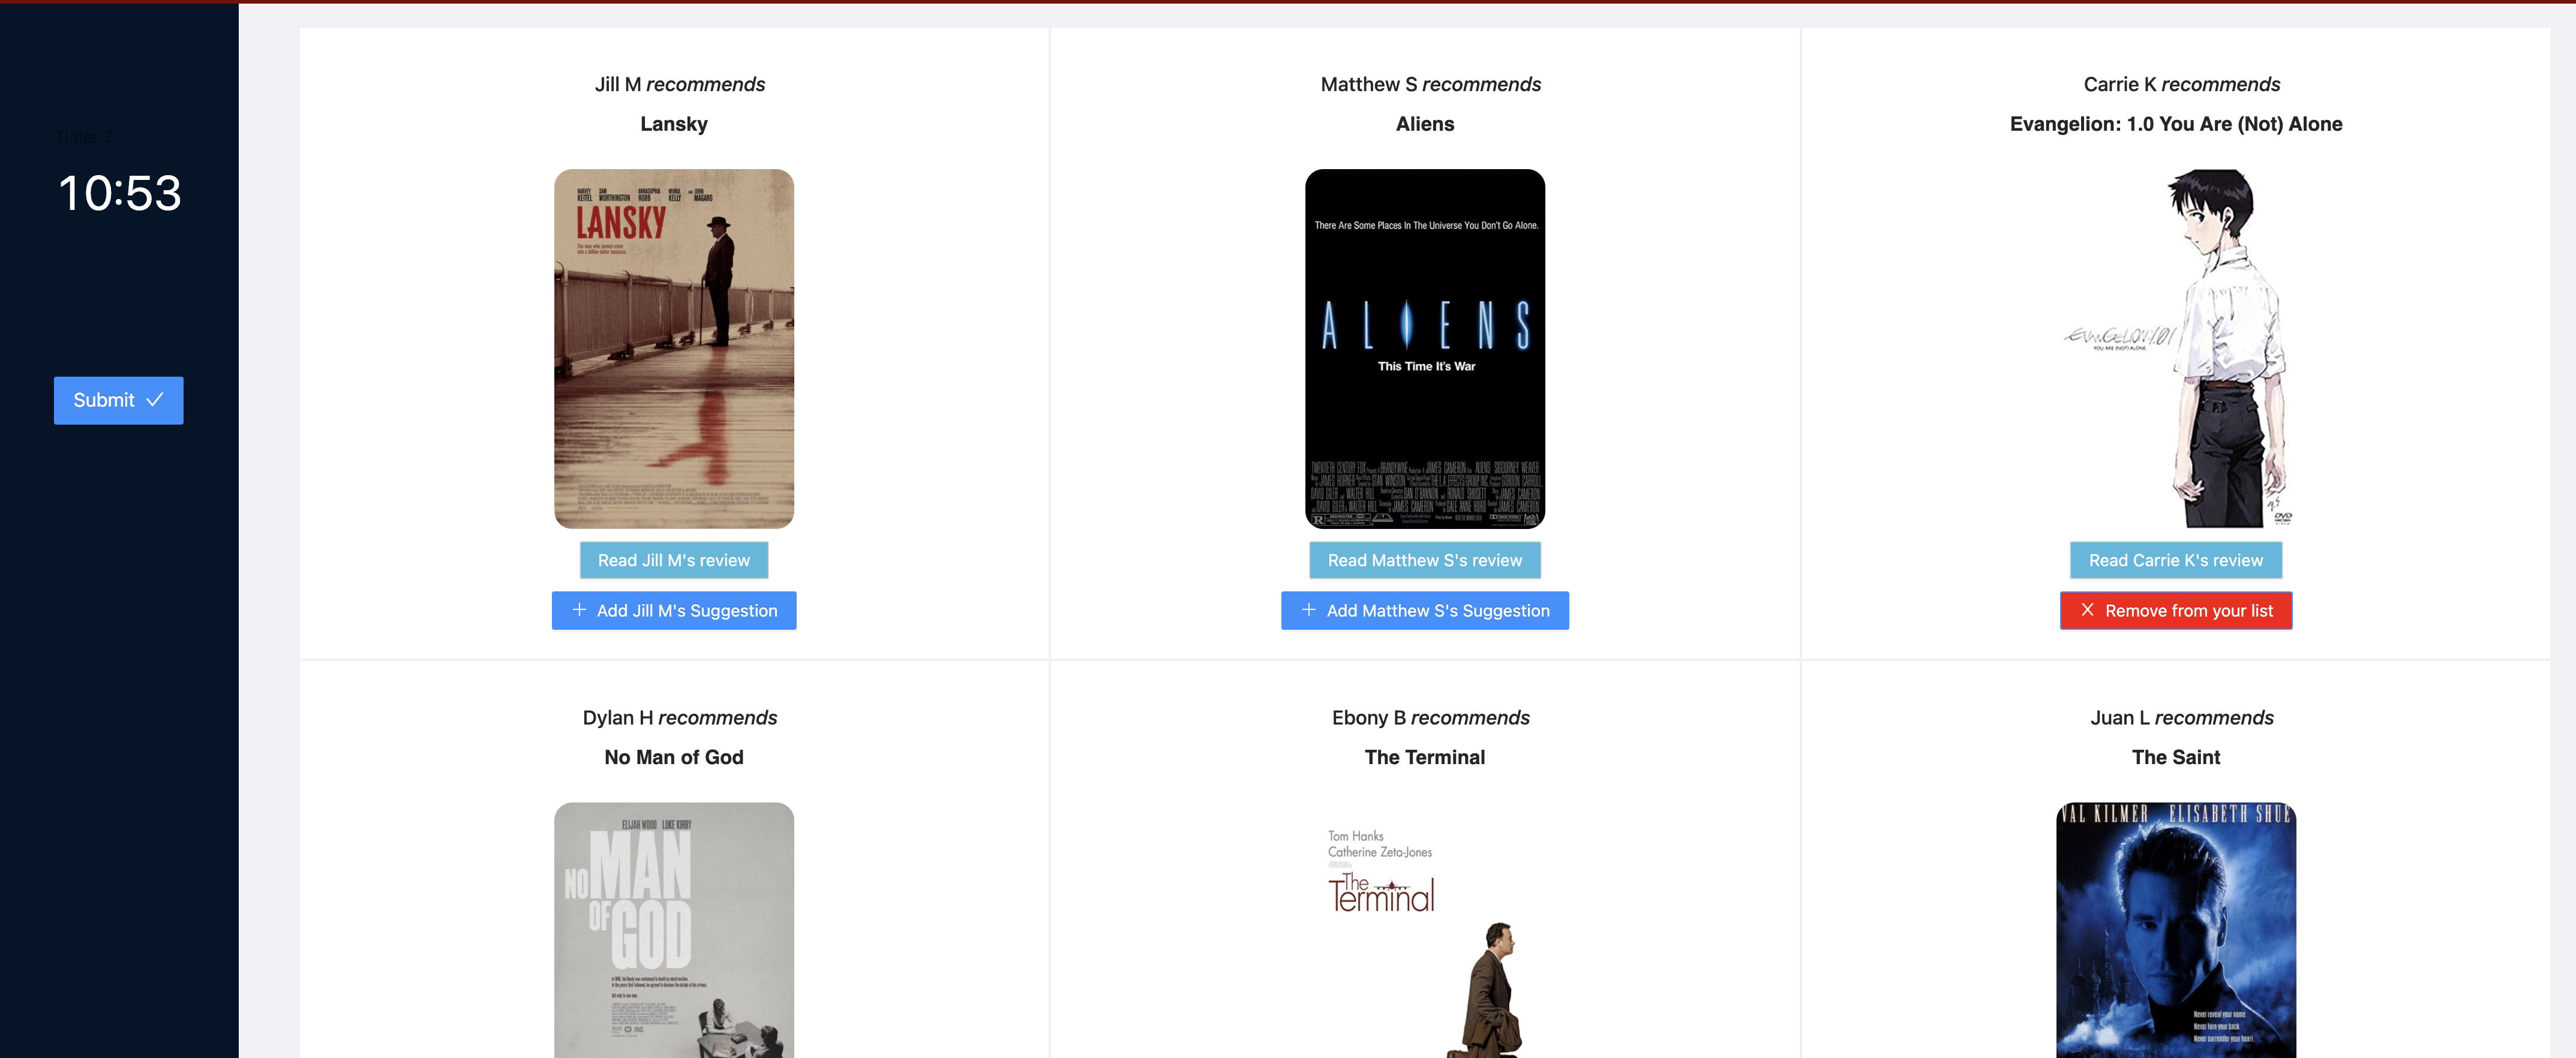
\includegraphics[width=1\linewidth]{Misc Screenshots/NonRushedScreenShotwithLoadMore.png}  
        \caption{Nonrushed Screen (After Selecting ``Load More'')}
         \label{fig:lab_nonrush_screenshot}
    \end{subfigure}
     \begin{subfigure}{.5\textwidth}
       \centering
        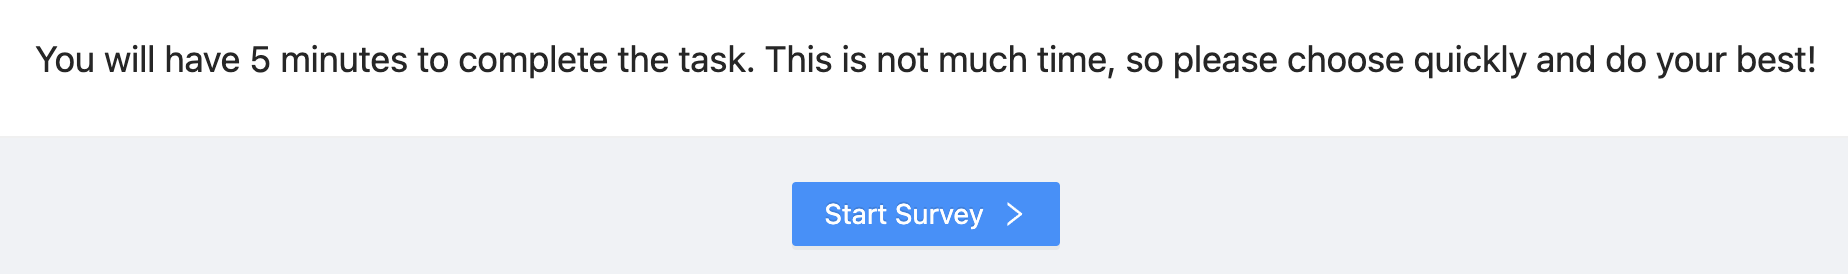
\includegraphics[width=1\linewidth]{Misc Screenshots/RushedTimeInstructions.png}  
        \caption{Rushed Time Instructions}
         \label{fig:lab_rush_instructions}
    \end{subfigure}
     \begin{subfigure}{.5\textwidth}
       \centering
        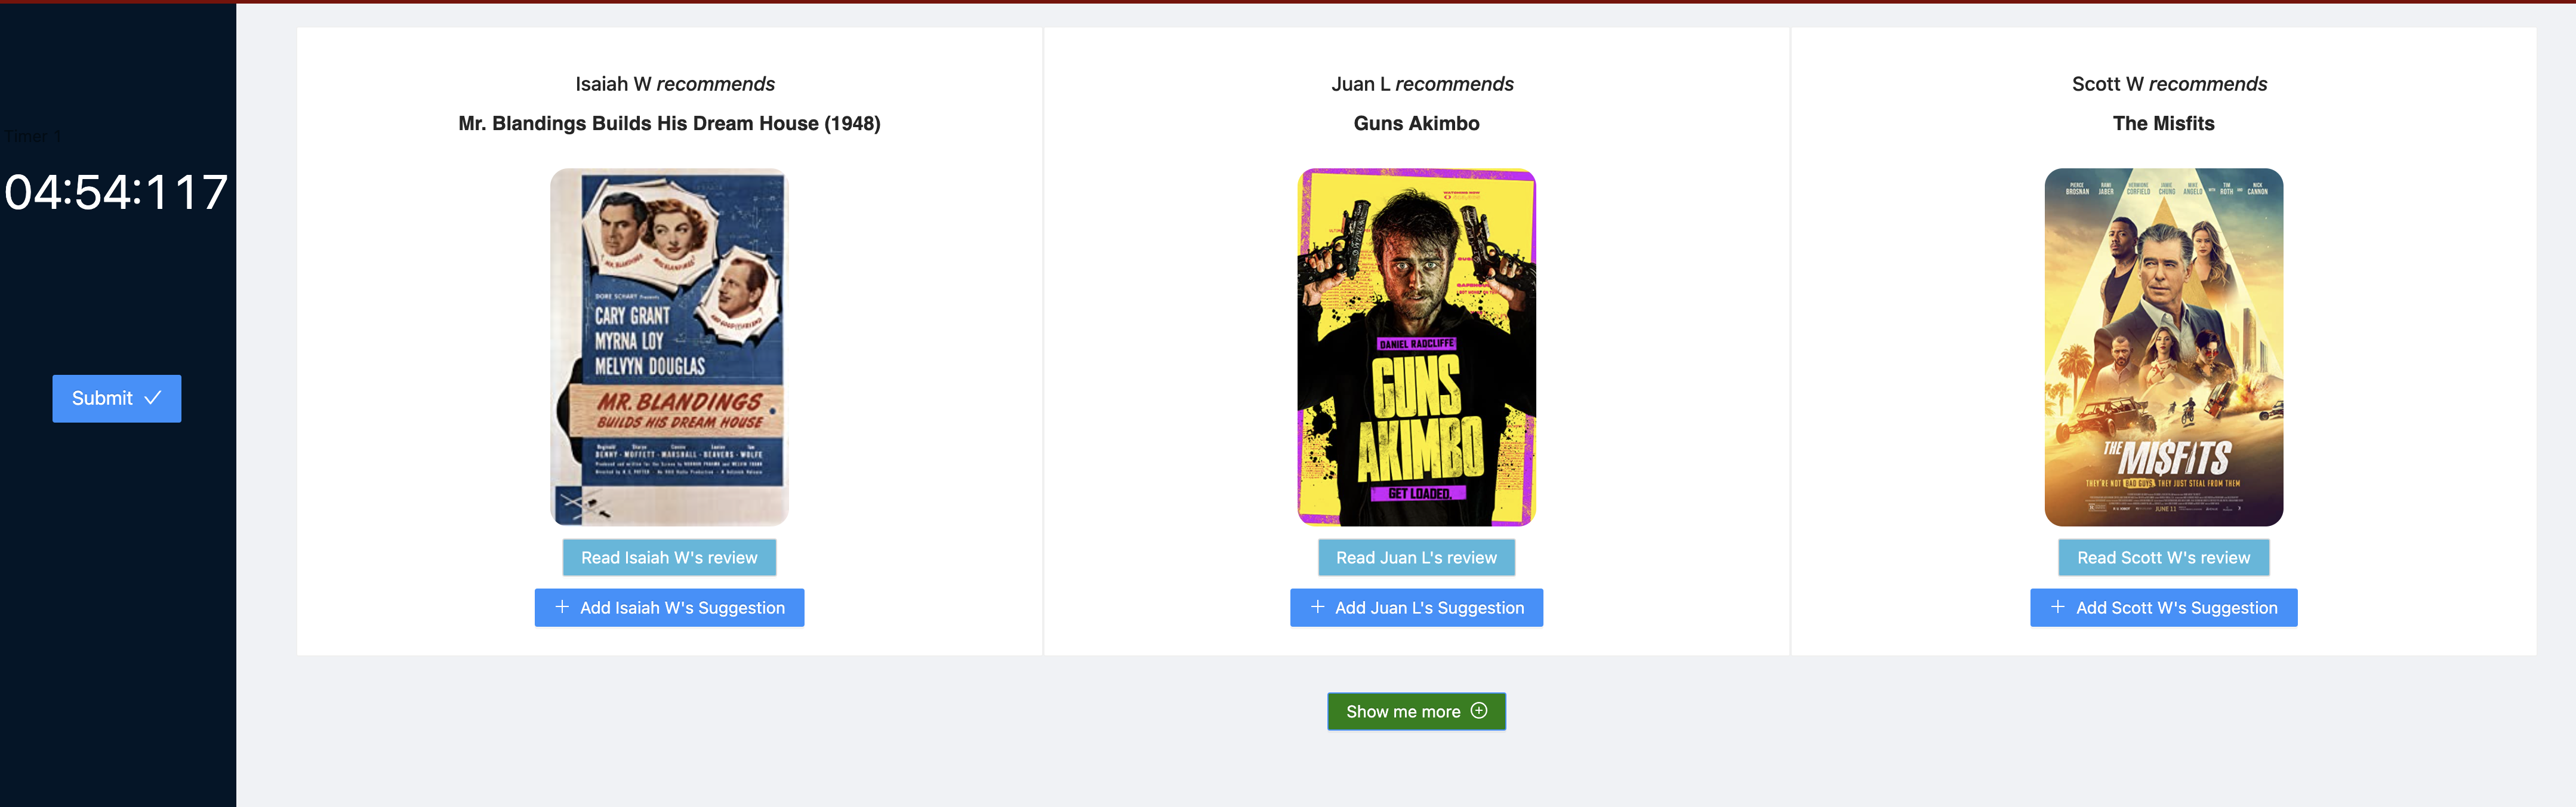
\includegraphics[width=1\linewidth]{Misc Screenshots/RushedScreenShot.png}  
        \caption{Rushed Screen}
         \label{fig:lab_rush_screenshot}
    \end{subfigure}

\footnotesize \textbf{Note:} Stuff about stuff
\end{figure}

%%%%%%%%%%
%%% LAB EXPERIMENTS: Summary Statistics
%%%%%%%%%%

\begin{table}[]
    \caption{Lab Experiment Subject Summary Statistics}
    \begin{center}
  %  \input{stff }
    \label{tab:samplab}
    \end{center}
\footnotesize \textbf{Note:} 
\end{table}

%%%%%%%%%%
%%% LAB EXPERIMENT 1 Results
%%%%%%%%%%

\begin{figure}[ht]
\caption{Lab Experiment 1 Results}
\label{fig:lab1}
    \begin{subfigure}{.5\textwidth} 
        \centering
       % 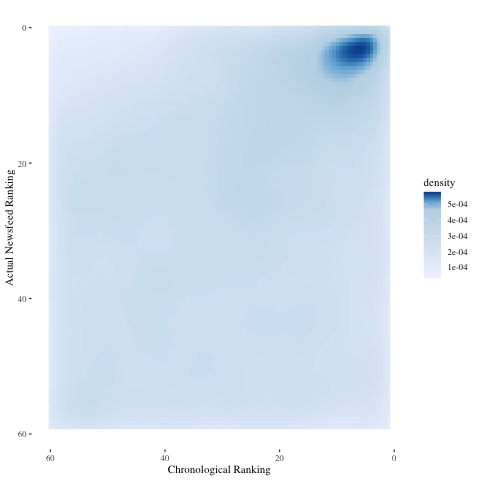
\includegraphics[width=1\linewidth]{Output/Graphs/Audit/Heatmaps/US NF chron rank by nf rank - smooth.jpg}   
        \caption{Click Results}
        \label{fig:lab1_click}
        \end{subfigure}
    \begin{subfigure}{.5\textwidth}
       \centering
       % 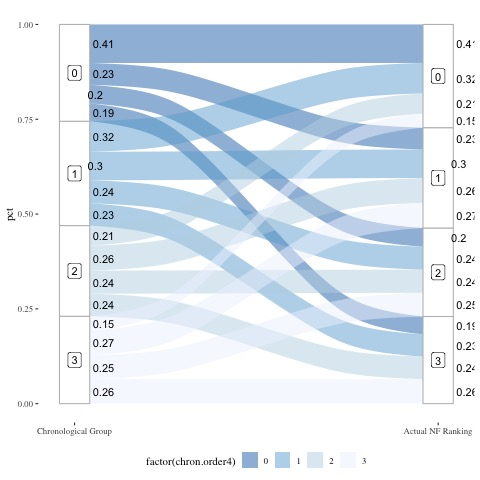
\includegraphics[width=1\linewidth]{Output/Graphs/Audit/Sankey flows/US NF chronology to actual.jpg}  
        \caption{Lab 1 Algorithm}
         \label{fig:lab1_algo}
    \end{subfigure}
=
\footnotesize \textbf{Note:} Stuff about stuff
\end{figure}

%%%%%%%%%%
%%% LAB EXPERIMENT 2 Results
%%%%%%%%%%

\begin{figure}[ht]
\caption{Lab Experiment 2 Results}
\label{fig:lab2}
    \begin{subfigure}{.5\textwidth} 
        \centering
       % 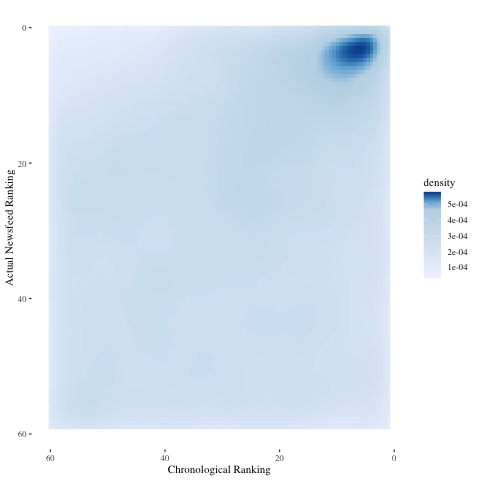
\includegraphics[width=1\linewidth]{Output/Graphs/Audit/Heatmaps/US NF chron rank by nf rank - smooth.jpg}   
        \caption{Click Results}
        \label{fig:lab2_click}
        \end{subfigure}
    \begin{subfigure}{.5\textwidth}
       \centering
       % 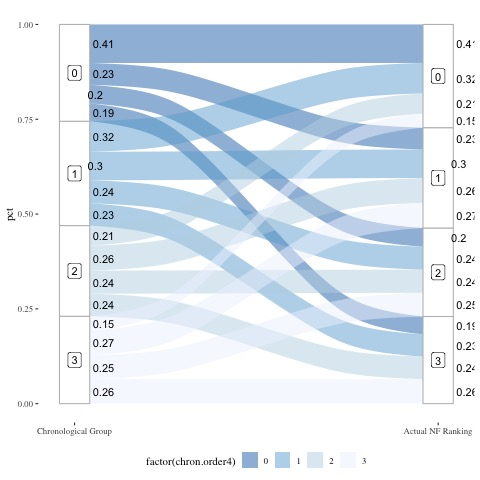
\includegraphics[width=1\linewidth]{Output/Graphs/Audit/Sankey flows/US NF chronology to actual.jpg}  
        \caption{Lab 2 Algorithm}
         \label{fig:lab2_algo}
    \end{subfigure}
=
\footnotesize \textbf{Note:} Stuff about stuff
\end{figure}

%%%%%%%%%%
%%% US FACEBOOK: Summary Statistics
%%%%%%%%%%


\begin{table}[]
    \caption{Facebook Subject Summary Statistics}
    \begin{center}
    {
\def\sym#1{\ifmmode^{#1}\else\(^{#1}\)\fi}
\begin{tabular}{l*{3}{c}}
\toprule
                    &\multicolumn{1}{c}{(1)}&\multicolumn{1}{c}{(2)}&\multicolumn{1}{c}{(3)}\\
                    &\multicolumn{1}{c}{Newsfeed}&\multicolumn{1}{c}{PYMK}&\multicolumn{1}{c}{Activity}\\
\midrule
Race of subject (RA)&            &            &            \\
\hspace{3mm} Asian  &       0.409&       0.445&       0.308\\
\hspace{3mm} Black  &       0.091&       0.087&       0.115\\
\hspace{3mm} Hispanic&       0.091&       0.073&       0.125\\
\hspace{3mm} Other Race&       0.014&       0.016&       0.000\\
\hspace{3mm} White  &       0.396&       0.379&       0.452\\
Race of Subject (Self Identification)&            &            &            \\
\hspace{3mm} Asian  &       0.385&       0.429&       0.260\\
\hspace{3mm} Black  &       0.071&       0.078&       0.077\\
\hspace{3mm} Hispanic&       0.066&       0.046&       0.087\\
\hspace{3mm} Other Race&       0.024&       0.023&       0.029\\
\hspace{3mm} White  &       0.353&       0.336&       0.423\\
\hspace{3mm} Two or more Races&       0.069&       0.062&       0.087\\
Gender              &            &            &            \\
 \hspace{3mm} Male  &       0.261&       0.269&       0.221\\
 \hspace{3mm} Female&       0.681&       0.676&       0.721\\
 \hspace{3mm} Non-binary&       0.027&       0.027&       0.019\\
Age                 &      26.639&      27.138&      26.090\\
Less than Bachelor's Degree&       0.379&       0.358&       0.385\\
Bachelor's Degree   &       0.346&       0.347&       0.317\\
Graduate Degree     &       0.224&       0.240&       0.260\\
Average Facebook Usage&            &            &            \\
\hspace{3mm} Hourly &       0.119&       0.123&       0.125\\
\hspace{3mm} Daily  &       0.517&       0.534&       0.481\\
\hspace{3mm} Weekly &       0.234&       0.224&       0.279\\
\hspace{3mm} Monthly&       0.074&       0.073&       0.067\\
\hspace{3mm} Yearly &       0.018&       0.014&       0.000\\
\hspace{3mm} Never  &       0.008&       0.005&       0.010\\
\hspace{3mm} Within past hour&       0.473&       0.486&       0.423\\
Last Facebook Log-in&            &            &            \\
\hspace{3mm} Within past day&       0.364&       0.349&       0.442\\
\hspace{3mm} Within past month&       0.030&       0.021&       0.029\\
\hspace{3mm} Within past week&       0.098&       0.112&       0.067\\
\hspace{3mm} Within past year&       0.005&       0.005&       0.000\\
Total Facebook Friends&     810.386&     836.215&     864.524\\
Mean NF Post Preference&       3.439&       3.338&       3.518\\
Standard Dev of NF Post Preference&       1.640&       1.625&       1.698\\
Mean PYMK Rec Familiarity&       2.351&       2.351&           .\\
Standard Dev of PYMK Rec Familiarity&       1.636&       1.636&           .\\
\midrule
Observations        &         662&         438&         104\\
\bottomrule
\end{tabular}
}

    \label{tab:sumstats_p}
    \end{center}
\footnotesize \textbf{Note:} 
\end{table}

%\input{Output/Tex/Summary Tables/US NF subjects by sample.tex}

%% Created by Amanda

\begin{table}[!htbp] \centering 
  \caption{} 
  \label{tab:outcomesumstats} 
\begin{tabular}{@{\extracolsep{5pt}} lcccc} 
\\[-1.8ex]\hline 
\hline \\[-1.8ex] 
&\multicolumn{3}{c}{Newsfeed Data} &\multicolumn{1}{c}{PYMK} \\\cmidrule(lr){2-4}\cmidrule(lr){5-5}\\
 & NF Sample & PYMK Sample & Behavior Sample & PYMK Sample\\ 
\hline \\[-1.8ex] 
N & 37347 & 25549 & 4680 & 25593 \\ 
mean..sd. & 3.41 $\pm$ 1.94 & 3.33 $\pm$ 1.92 & 3.44 $\pm$ 1.97 & 2.35$\pm$1.86 \\ 
Median..IQR. & 3 (2.00, 5.00) & 3 (2.00, 5.00) & 3.00 (2.00, 5.00) & 1(1.00, 3.00) \\ 
X7s..Most.preferred. & 8.12\%   & 7.47\%   & 9.12\%   & 5.29\% \\ 
X6s & 9.72\%   & 9.00\%   & 9.79\%   & 4.34\% \\ 
X5s & 13.65\%   & 13.35\%   & 12.78\%   & 6.87\% \\ 
X4s & 14.03\%   & 13.86\%   & 14.47\%   & 7.92\% \\ 
X3s & 15.17\%   & 15.40\%   & 15.00\%   & 9.13\% \\ 
X2s & 16.58\%   & 17.06\%   & 15.49\%   & 12.06\% \\ 
X1s..Least.preferred. & 22.73\%   & 23.86\%   & 23.35\%   & 54.40\% \\ 
Asian & 20.02\%   & 21.21\%   & 17.12\%   & 30.87\%\\ 
Black.AA & 7.98\%   & 8.79\%   & 7.09\%   & 8.87\% \\ 
Hispanic & 7.92\%   & 7.42\%   & 8.38\%   & 9.06\% \\ 
Other & 25.01\%   & 24.29\%   & 27.74\%   & 3.54\% \\ 
White & 39.07\%   & 38.29\%   & 39.68\%   & 47.66\% \\ 
Multiple.races & 1.08\%   & 0.97\%   & 0.60\%  & 1.00\%\\ 
% mean..sd..1 & 1.19 $\pm$ 2.97 & 1.22 $\pm$ 3.30 & 1.20 $\pm$ 2.60 & \\ 
% Median..IQR..1 & 0.58 (0.08, 2.00) & 0.58 (0.08, 1.00) & 0.67 (0.12, 2.00) & 0.0 \\ 
Same.Race.Rate & 0.60 & 0.60 & 0.58 & 0.58\\ 
Same.Gender.Rate & 0.60 & 0.60 & 0.61 & 0.57 \\ 
Human.Rate & 0.77 & 0.78 & 0.74 & NA\\ 
Group.Post.Rate & 0.33 & 0.33 & 0.40 & NA \\ 
Common Friends &  & & &  22.93$\pm$ 37.90 \\
\hline \\[-1.8ex] 
\end{tabular} 
\end{table} 


\begin{table}[]
\caption{Summary Statistics on Collected Outcomes}
    \begin{center}
    {
\def\sym#1{\ifmmode^{#1}\else\(^{#1}\)\fi}
\begin{tabular}{l*{7}{c}}
\toprule
                    &\multicolumn{3}{c}{Newsfeed Posts}    &\multicolumn{3}{c}{PYMK Recommendations}&\multicolumn{1}{c}{\shortstack{Last 10 \\Interactions}}\\\cmidrule(lr){2-4}\cmidrule(lr){5-7}\cmidrule(lr){8-8}
                    &\multicolumn{1}{c}{(1)}&\multicolumn{1}{c}{(2)}&\multicolumn{1}{c}{(3)}&\multicolumn{1}{c}{(4)}&\multicolumn{1}{c}{(5)}&\multicolumn{1}{c}{(6)}&\multicolumn{1}{c}{(7)}\\
                    &\multicolumn{1}{c}{All}&\multicolumn{1}{c}{Ingroup}&\multicolumn{1}{c}{Outgroup}&\multicolumn{1}{c}{All}&\multicolumn{1}{c}{Ingroup}&\multicolumn{1}{c}{Outgroup}&\multicolumn{1}{c}{All}\\
\midrule
Ingroup (Race)      &       0.601&            &            &       0.585&            &            &       0.683\\
Race of Poster/Rec  &            &            &            &            &            &            &            \\
\hspace{3mm} Asian  &       0.257&            &            &       0.306&            &            &            \\
\hspace{3mm} Black  &       0.102&            &            &       0.086&            &            &            \\
\hspace{3mm} Hispanic&       0.100&            &            &       0.089&            &            &            \\
\hspace{3mm} Other Race&       0.028&            &            &       0.035&            &            &            \\
\hspace{3mm} White  &       0.499&            &            &       0.469&            &            &            \\
Preference--1st Quartile&       0.249&       0.247&       0.253&       0.250&       0.238&       0.266&            \\
Preference--2nd Quartile&       0.251&       0.249&       0.253&       0.250&       0.249&       0.251&            \\
Preference--3rd Quartile&       0.250&       0.254&       0.245&       0.250&       0.253&       0.246&            \\
Preference--4th Quartile&       0.250&       0.251&       0.249&       0.250&       0.259&       0.238&            \\
Ranking             &      29.265&      28.777&      30.000&      30.350&      30.380&      30.307&            \\
In First 10 Posts/Recs&       0.183&       0.192&       0.169&       0.168&       0.167&       0.170&            \\
Post to Group       &       0.365&            &            &            &            &            &            \\
Days Ago Posted     &       1.134&       1.120&       1.156&            &            &            &      18.120\\
Mutual Friends      &            &            &            &      22.933&      21.902&      24.385&            \\
Liked/Reacted to Post&            &            &            &            &            &            &       0.836\\
Commented on Post   &            &            &            &            &            &            &       0.173\\
\midrule
Observations        &       28747&       17271&       11476&       25593&       14969&       10624&         908\\
\bottomrule
\end{tabular}
}

    \label{tab:sumstats_o}
    \end{center}
\footnotesize \textbf{Note:} 
\end{table}

%%%%%%%%%%
%%% US: NF
%%%%%%%%%%

%%% NF Heatmap and Sankey: Chron vs Algorithm and Pref vs Algorithm %%%
\begin{figure}[ht]
\caption{Relationship between Newsfeed Algorithmic Ranking and Chronology and User Stated Preferences }
\label{fig:nf}
    \begin{subfigure}{.5\textwidth} 
        \centering
        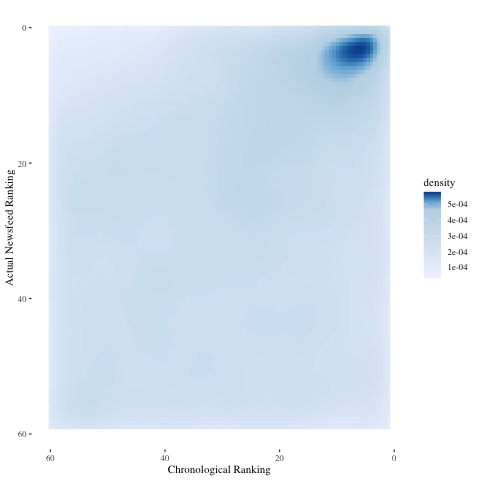
\includegraphics[width=1\linewidth]{Output/Graphs/Audit/Heatmaps/US NF chron rank by nf rank - smooth.jpg}   
        \caption{Relative Intensity of Posts by Chronological Ranking and Algorithmic Ranking}
        \label{fig:nftime_hm}
        \end{subfigure}
    \begin{subfigure}{.5\textwidth}
       \centering
        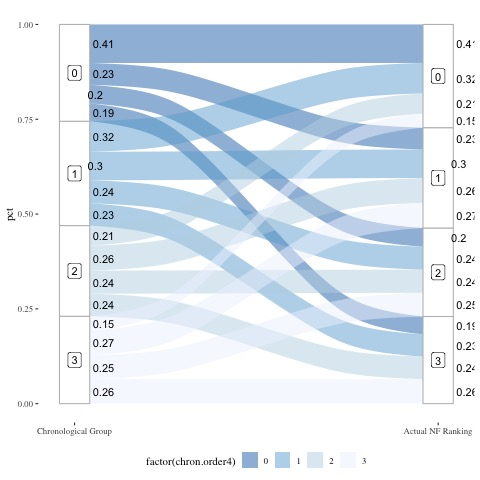
\includegraphics[width=1\linewidth]{Output/Graphs/Audit/Sankey flows/US NF chronology to actual.jpg}  
        \caption{Flows from Chronological Ranking Quartile to Algorithmic Ranking}
         \label{fig:nftime_s}
    \end{subfigure}

   \begin{subfigure}{.5\textwidth} 
        \centering
        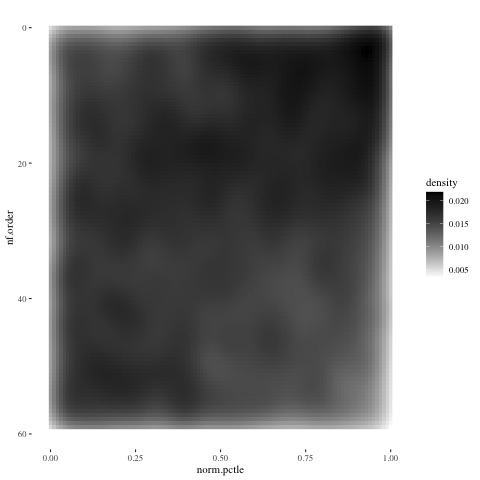
\includegraphics[width=1\linewidth]{Output/Graphs/Audit/Heatmaps/US NF norm pref rank by nf rank - smooth.jpg}  
        \caption{Relative Intensity of Posts by Normalized Preference  and Algorithmic Ranking}
        \label{fig:nfpref_hm}
        \end{subfigure}
    \begin{subfigure}{.5\textwidth}
        \centering
        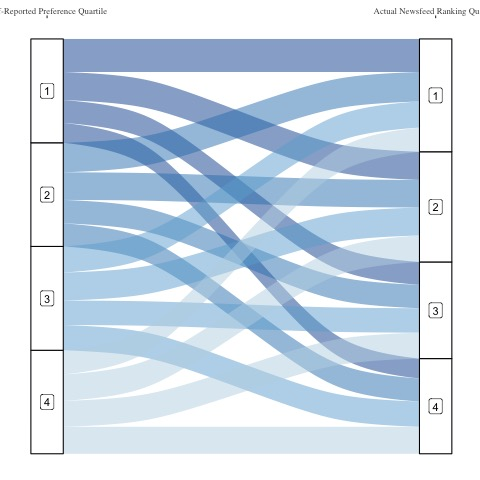
\includegraphics[width=1\linewidth]{Output/Graphs/Audit/Sankey flows/US NF norm quartile to actual.jpg}  
        \caption{Flows from Normalized Preference Quartile to Algorithmic Ranking}
        \label{fig:nfpref_s}
    \end{subfigure}

\footnotesize \textbf{Note:} Figures (a) and (c) are heatmaps which show that actual Newfeed algorithmic ranking (1-60) on the Y-axis and either chronological ranking (1-60)  or percentiles of normalized preference distribution (1-100) on the X-axis. The heatmaps are smoothed using a bivariate normal kernel density estimator. Figures (b) and (d) show flows from quartiles of the chronology ranking or preference distribution (on the left) to quartiles of the actual Newsfeed algorithmic ranking (on the right). The width of the bands represents the proportion in that flow.
\end{figure}



%%% NF in-group Posts %%%
\begin{figure}[ht]
\caption{Relationship between Newsfeed Algorithmic Ranking and in-group Status of Posts}
\label{fig:nf_bygroup}
    \begin{subfigure}{.5\textwidth} 
        \centering
        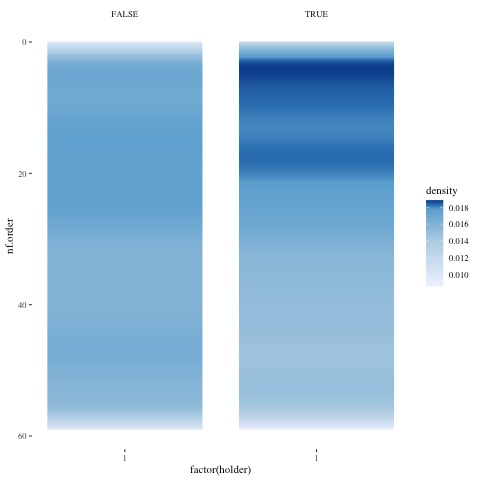
\includegraphics[width=1\linewidth]{Output/Graphs/Audit/Heatmaps/US NF nf rank by ingroup - smooth.jpg}  
        \caption{Relative Intensity of Posts by in-group Status and Algorithmic Ranking}
        \label{fig:nf_bygroup_hm}
        \end{subfigure}
    \begin{subfigure}{.5\textwidth}
        \centering
        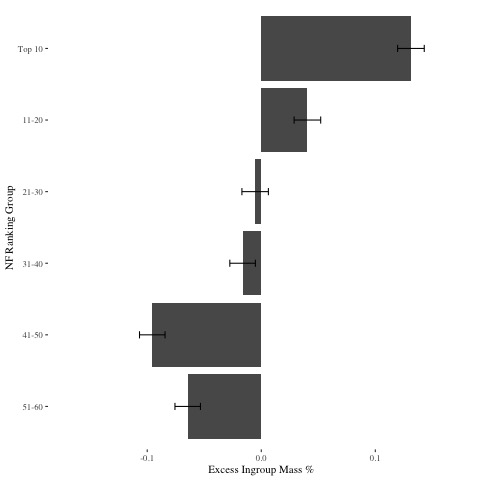
\includegraphics[width=.9\linewidth]{Output/Graphs/Audit/Excess Mass/US NF excess mass by ranking group.jpg}  
        \caption{Excess Mass of in-group Posts by Newsfeed Algorithmic Ranking}
        \label{fig:nf_bygroup_em}
    \end{subfigure}

\footnotesize \textbf{Note:} Figure (a) shows the relative intensity of algorithmic ranking for each group identity (in-group vs outgroup). Figure (b) shows the excess mass of ingroup posts by algortihmic ranking in bins of 10. Excess mass is the ratio between the fraction of ingroup posts within a bin and the fraction of outgroup posts within a bin, effectively calculating the extent to which ingroup posts are over (or under) represented in a bin.
\end{figure}

%%% NF Ranking by preference %%%
\begin{figure}[ht]
\caption{Relationship between Newsfeed Algorithmic Ranking and in-group Status conditional on Subject Explicit Preference}
\label{fig:nf_main}
    \begin{subfigure}{.5\textwidth} 
        \centering
            % include first image
        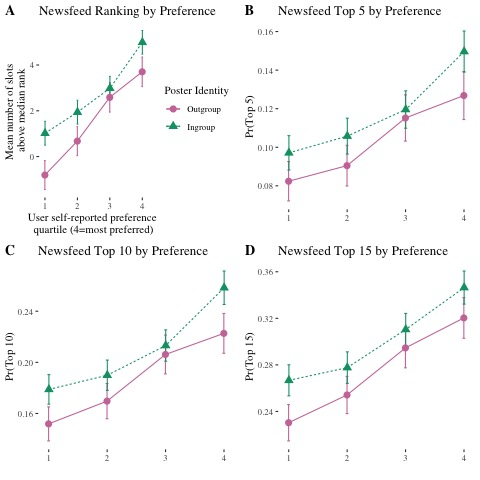
\includegraphics[width=1\linewidth]{Output/Graphs/Audit/Ranking line graphs/US NF all outcomes panel by norm preference by ingroup.jpg} 
        \caption{Ranking Boost Above Median Rank}
        \label{fig:nf_line}
        \end{subfigure}
    \begin{subfigure}{.5\textwidth}
        \centering
        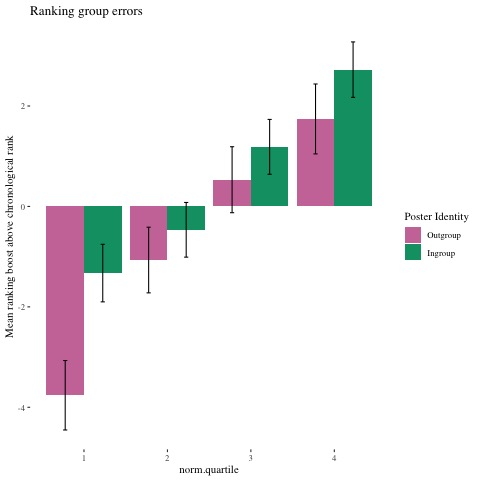
\includegraphics[width=1\linewidth]{Output/Graphs/Audit/Misranking relative to expectation/Chronological expectation/US NF by norm preference.jpg}  
        \caption{Ranking Boost Above Chronological Rank}
        \label{fig:nf_rankingboost}
    \end{subfigure}

\footnotesize \textbf{Note:} Normalized subject explicit preference quartile is the across subject quartile of within subject z-scores for stated preference for a post. Each subjects ratings were mean-centered and then divided by the subject's standard deviation of responses. The resulting distribution was then split into four equally sized bins. The mean number of slots above median rank is the average ranking (1-60) minus the median of the distribution (30.5). Prob(Top \textit{m}) is the percent of posts with algorithm rank $\le$\textit{m}. The mean ranking above chronological rank is the average difference between where a post would fall in a chronological rank and where it was actually ranked in the newsfeed, where positive numbers indicate that the algorithm sorted the post closer to the top than a chronological sort would have.
\end{figure}

%%%%%%%%%%
%%% US: PYMK
%%%%%%%%%%

%%% NF Heatmap and Sankey: Chron vs Algorithm and Pref vs Algorithm %%%
\begin{figure}[ht]
\caption{Relationship between PYMK Algorithmic Ranking and Chronology and User Stated Preferences}
\label{fig:pymk}
    \begin{subfigure}{.5\textwidth} 
        \centering
        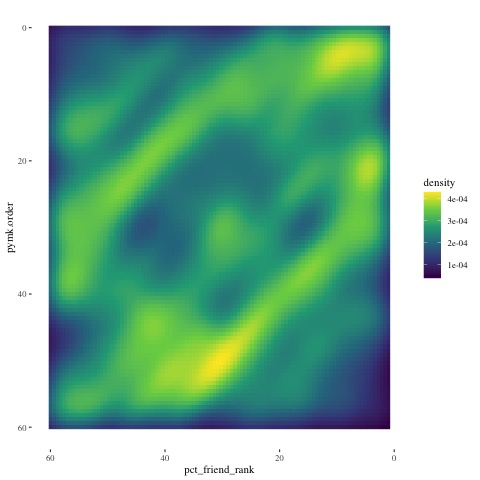
\includegraphics[width=1\linewidth]{Output/Graphs/Audit/Heatmaps/US PYMK pct friends by pymk rank - smooth.jpg}   
        \caption{Relative Intensity of Recommendations by Percent Mutual Friends and Algorithmic Ranking}
        \label{fig:pymkfriend_hm}
        \end{subfigure}
    \begin{subfigure}{.5\textwidth}
        \centering
        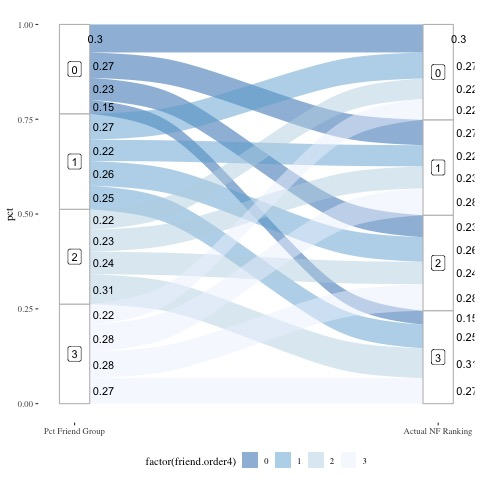
\includegraphics[width=1\linewidth]{Output/Graphs/Audit/Sankey flows/US PYMK pct friend to actual.jpg}  
        \caption{Flows from Percent Mutual Friends Quartile to Algorithmic Ranking}
        \label{fig:pymkfriend_s}
    \end{subfigure}

   \begin{subfigure}{.5\textwidth} 
        \centering
        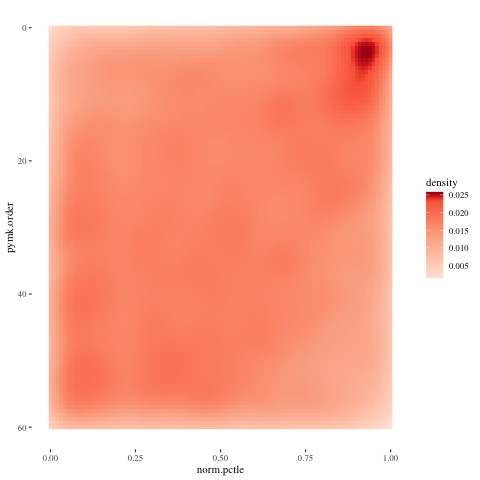
\includegraphics[width=1\linewidth]{Output/Graphs/Audit/Heatmaps/US PYMK norm pref rank by pymk rank - smooth.jpg}  
        \caption{Relative Intensity of Recommendations by Normalized Familiarity and Algorithmic Ranking}
        \label{fig:pymkpref_hm}
        \end{subfigure}
    \begin{subfigure}{.5\textwidth}
        \centering
        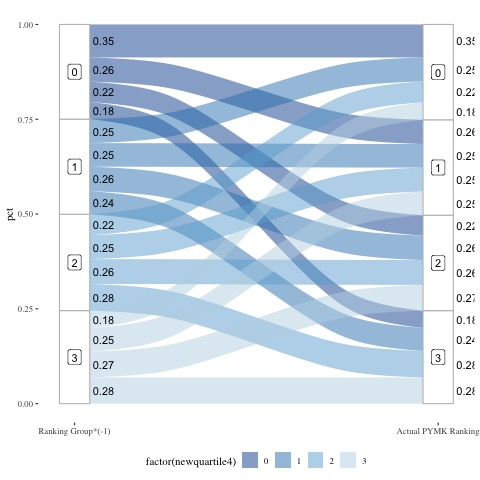
\includegraphics[width=1\linewidth]{Output/Graphs/Audit/Sankey flows/US PYMK norm quartile to actual.jpg}  
        \caption{Flows from Normalized Familiarity Quartile to Algorithmic Ranking}
        \label{fig:pymkpref_s}
    \end{subfigure}
    
\footnotesize \textbf{Note:} 
\end{figure}


%%% PYMK in-group Posts %%%
\begin{figure}[ht]
\caption{Relationship between PYMK Algorithmic Ranking and in-group Status of Posts}
\label{fig:pymk_bygroup}
    \begin{subfigure}{.5\textwidth} 
        \centering
        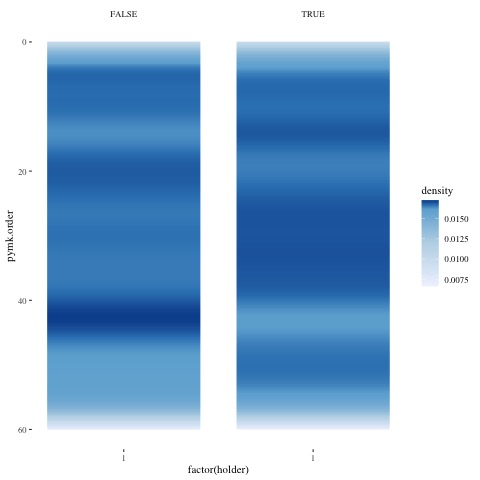
\includegraphics[width=1\linewidth]{Output/Graphs/Audit/Heatmaps/US PYMK pymk rank by ingroup - smooth.jpg}  
        \caption{Relative Intensity of Posts by In-group status and Algorithmic Ranking}
        \label{fig:pymk_bygroup_hm}
        \end{subfigure}
    \begin{subfigure}{.5\textwidth}
        \centering
        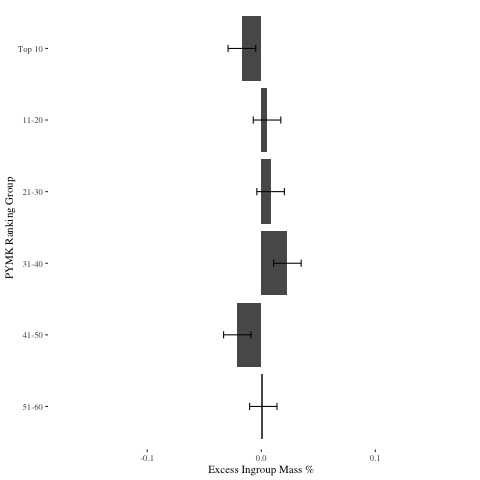
\includegraphics[width=.9\linewidth]{Output/Graphs/Audit/Excess Mass/US PYMK excess mass by ranking group.jpg}  
        \caption{Excess Mass of In-group Posts by PYMK Algorithmic Ranking}
        \label{fig:pymk_bygroup_em}
    \end{subfigure}

\end{figure}

%%% PYMK Ranking by preference %%%
\begin{figure}[ht]
\caption{Relationship between PYMK Algorithmic Ranking and In-group Status conditional on Subject Familiarity}
\label{fig:pymk_main}
    \begin{subfigure}{.5\textwidth} 
        \centering
            % include first image
        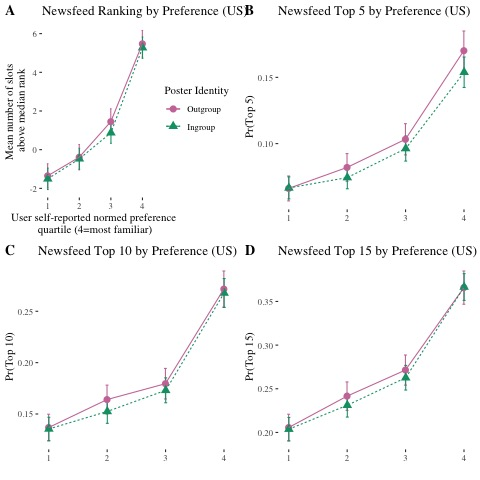
\includegraphics[width=1\linewidth]{Output/Graphs/Audit/Ranking line graphs/US PYMK all outcomes panel by norm preference by ingroup.jpg} 
        \caption{Ranking Boost Above Median Rank}
        \label{fig:pymk_line}
        \end{subfigure}
    \begin{subfigure}{.5\textwidth}
        \centering
        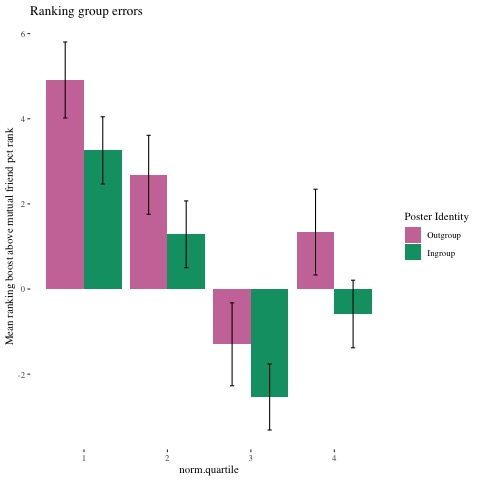
\includegraphics[width=1\linewidth]{Output/Graphs/Audit/Misranking relative to expectation/Mutual friends expectation/US PYMK by norm pref.jpg}  
        \caption{Ranking Boost Above Chronological Rank}
        \label{fig:pymk_rankingboost}
    \end{subfigure}
\footnotesize \textbf{Note:} 
\end{figure}

%%%%%%%%%%
%%% US: AUTO
%%%%%%%%%%

\begin{figure}
\caption{Deliberateness}
  \begin{subfigure}{.5\textwidth} 
        \centering
        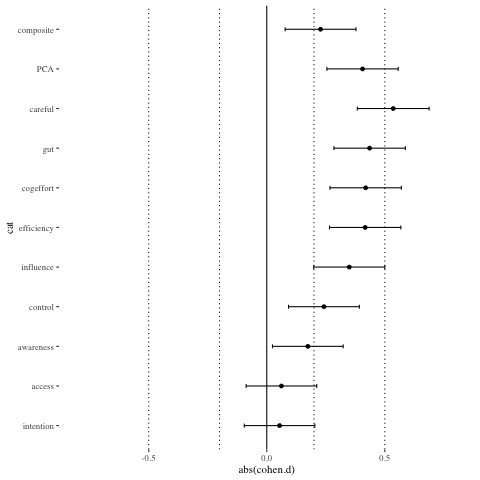
\includegraphics[width=1\linewidth]{Output/Graphs/Experiments/Automaticity/standardized effect sizes.jpg} 
        \caption{Standardized Effect Sizes}
        \label{fig:auto_effsize}
    \end{subfigure}
    \begin{subfigure}{.5\textwidth} 
        \centering
        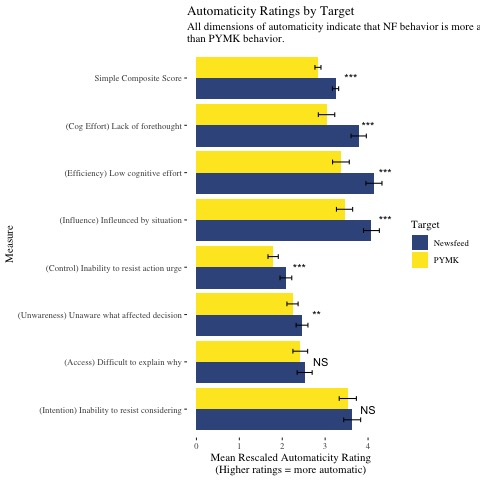
\includegraphics[width=1\linewidth, trim={0cm 0 3cm 2cm}, clip]{Output/Graphs/Experiments/Automaticity/composite score and components.jpg}  
        \caption{Likerts (and average composite)}
        \label{fig:auto_likerts}
        
    \end{subfigure}
    \begin{subfigure}{.5\textwidth}
        \centering
        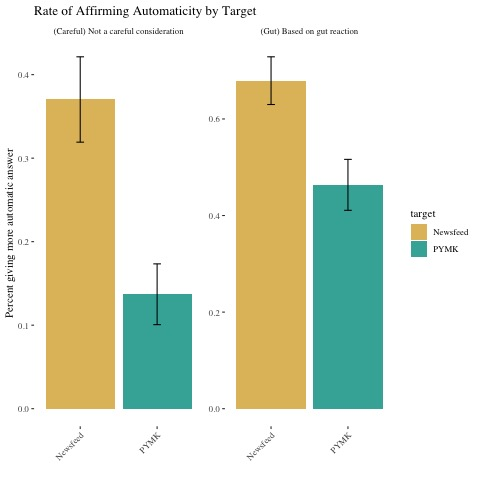
\includegraphics[width=1\linewidth, trim={0cm 0 3cm 2cm}, clip]{Output/Graphs/Experiments/Automaticity/bar chart binary measures.jpg} 
        \caption{Just the binaries}
        \label{fig:auto_binaries}
    \end{subfigure}
    \begin{subfigure}{.5\textwidth}
        \centering
        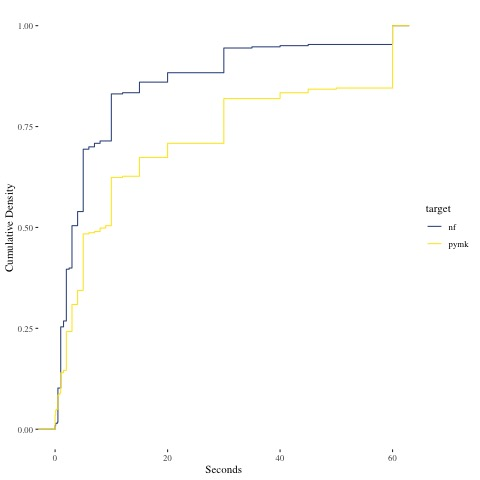
\includegraphics[width=1\linewidth, trim={0cm 0 2cm 0cm}, clip]{Output/Graphs/Experiments/Automaticity/speed cdf - bin over 60.jpg}  
        \caption{Speed (time to decide in seconds) CDF}
        \label{fig:auto_cdf}
    \end{subfigure}
\label{fig:auto}
\footnotesize \textbf{Note:} We collected 10 measures of deliberateness in making decisions in response to the newsfeed algortihm and the PYMK algorithm. The mean responses for the 7 Likert response questions along with the mean response across questions (Simple Composite Score) is shown in Figure (b).  The percent of respondents agreeing with the more automatic option of the two binary questions is shown in Figure (c). The CDF of self-reported typical time to decide to take an action (top-coded at 60 seconds) is shown in Figure (d). The standardized effect size is the mean response for the newsfeed and the mean response for PYMK divided by the pooled standard deviation. Higher values indicate more automatic for all questions except time where more seconds indicates more deliberation.
\end{figure}

% \begin{figure}
% \caption{Deliberateness}
%   \begin{subfigure}{.5\textwidth} 
%         \centering
%         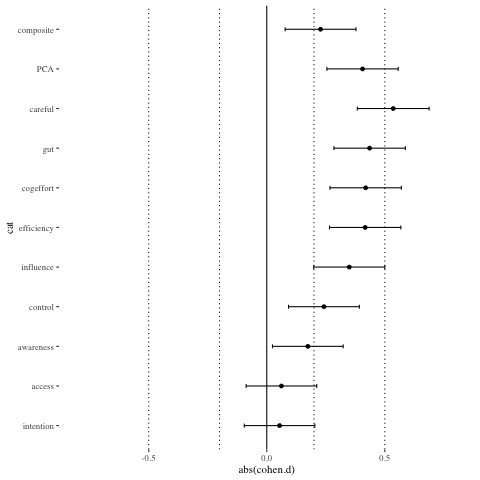
\includegraphics[width=1\linewidth, height=10cm, angle=270]{Output/Graphs/Experiments/Automaticity/standardized effect sizes.jpg} 
%         \caption{Standardized Effect Sizes}
%         \label{fig:auto_effsize}
%     \end{subfigure} \qquad
%     \begin{subfigure}{.5\textwidth} 
%         \centering
%         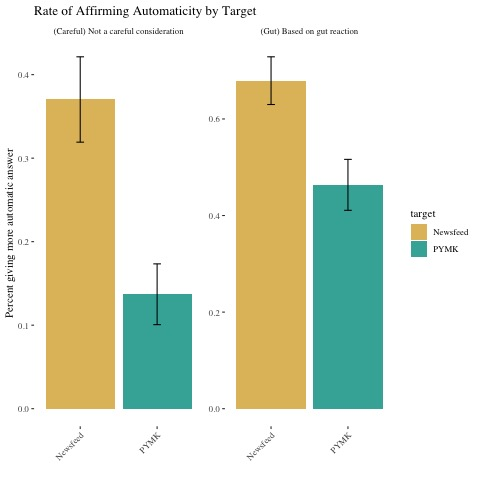
\includegraphics[width=1\linewidth, height=4cm, trim={0cm 0 3cm 1cm}, clip]{Output/Graphs/Experiments/Automaticity/bar chart binary measures.jpg} 
%         \caption{Just the binaries}
%         \label{fig:auto_binaries}
%         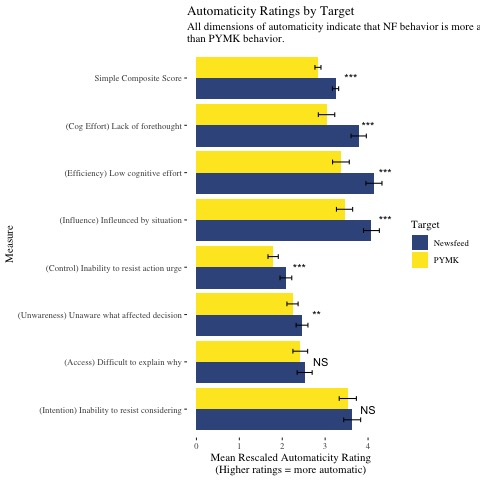
\includegraphics[width=1\linewidth, height=4cm, trim={0cm 0 3cm 2cm}, clip]{Output/Graphs/Experiments/Automaticity/composite score and components.jpg}  
%          \caption{Likerts (and average composite)}
%         \label{fig:auto_likerts}
%           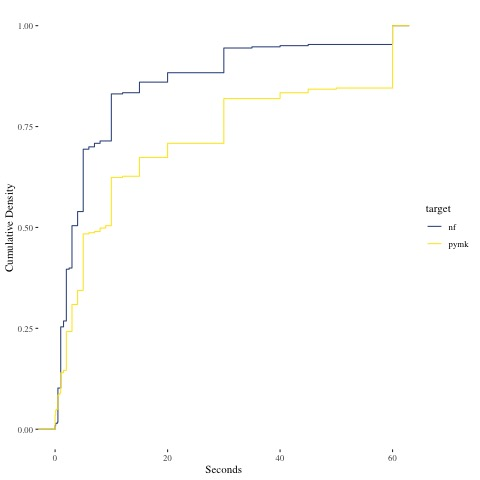
\includegraphics[width=1\linewidth, height=4cm, trim={0cm 0 2cm 0cm}, clip]{Output/Graphs/Experiments/Automaticity/speed cdf - bin over 60.jpg}  
%         \caption{Speed (time to decide in seconds) CDF}
%         \label{fig:auto_cdf}
%     \end{subfigure}
    
% \label{fig:auto}
% \footnotesize \textbf{Note:} 
% \end{figure}

%%%%%%%%%%
%%% US: Interactions
%%%%%%%%%%
\begin{figure}[!h]
    \caption{Share Recent Interactions In-Group versus Newsfeed Posts}
    \label{fig:behavior}
    \begin{center}
    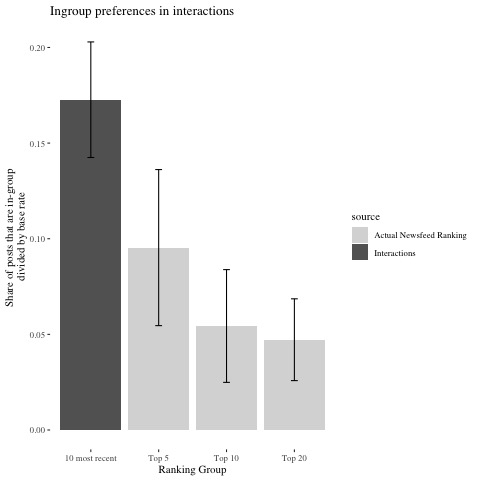
\includegraphics[scale=.7, trim={0 0 0cm 2cm}, clip]{Output/Graphs/Audit/Interactions/US preferences reactions and actual rankings above base rate.jpg}
    \end{center}
\footnotesize 
\textbf{Note:} 
\end{figure}

%%%%%%%%%% %%%%%%%%%% %%%%%%%%%% 
%%%%%%%%%% Appendix %%%%%%%%%%
%%%%%%%%%% %%%%%%%%%% %%%%%%%%%% 
\FloatBarrier
\clearpage
\appendix
\renewcommand\thefigure{\thesection.\arabic{figure}}
\renewcommand\thetable{\thesection.\arabic{table}}
\counterwithin{table}{section}


%%%%%% Materials and Methods Appendix %%%%%% 
\section{Lab Experiment Materials and Methods}\label{app:labmaterials}

\section{Facebook Materials and Methods}\label{app:materials}

We collected data from XX subjects over six sequential waves between March XX, 2020 and October XX, 2020. Over four waves we recruited 466 subjects through the CDR (US); In a single wave we recruited 196 subjects through HDSL (US). All waves share the same basic structure in which 1) subject privately completes a self-assessment, 2) enumerator guides each subject through the Newsfeed while recording information about each post and 3) enumerator guides subject through some additional data collection.
%; In a single wave we recruited 198 subjects through CSBC (India).

Data from each subject was collected in a single one-on-one Zoom session with an enumerator which lasted approximately one hour on average. After the data collection was completed, subjects were sent a link to access their payment of \$20 (\$10 in India).

\subsection{Wave Overview}
\begin{itemize}
    \item Wave 1 - CDR, NF + PYMK, 242
    \item Wave 2 - HDSL, NF + PYMK, 196
   % \item Wave 3 - India, NF + PYMK, 198
    \item Wave 4 - CDR, NF + Recent Activity, 54
    \item Wave 5 - CDR, NF (connectedness), 120
    \item Wave 6 - CDR, NF (about) + Recent Activity, 50
\end{itemize}

\subsection{Waves 1-3}

Waves 1-3 were nearly identical, each wave was on a different population. Because waves 1 and 2 were in the US, the group membership was based on perceived race, whereas wave 3 in India collected group membership based on perceived religion.

\subsubsection{Part I: Subject Categorization} After joining a Zoom call with an RA, subjects are asked to fill out a Qualtrics survey. In the survey, subjects are asked to describe their demographics and Facebook usage. As a main variable in our study, the assessment of the in-group is paramount. US subjects are shown the seven race and ethnicity categories used in the US Census and are given the option to check as many boxes as they like. Indian subjects are asked to report their religion.

While the subject fills out the survey, the enumerator makes her best assessment of the subject’s in-group (race in the US; religion in India), using up to two categories. Neither the subject nor the enumerator is aware of the assessment that the other has made. This protocol has the advantage of allowing us to observe how much alignment there is between how subjects self-identify and how they are perceived.

\subsubsection{Part II: Newsfeed} Users open their Facebook account and share their screen with the RA. Then, scrolling sequentially through each post in the Newsfeed, the subject answers exactly one question about each post: “There are more posts than Facebook can possibly show you. How would you rate this post on a scale from 1-7 where 1 means ‘can skip’ and 7 means ‘definitely want to see’.” In addition to recording the explicit preference, the enumerator assesses and records the perceived race of the poster of the content as well some other details of the post such as how long ago it was posted and whether it was posted to a group. The exact data being recorded by the enumerator are unknown to the subject. This continues for the first 60 non-sponsored posts.

\subsubsection{Part III: People You May Know} Subjects then navigate to the Facebook recommender for new friends, entitled “People You May Know” (PYMK). The procedure for this section is similar to that in Part II. The subject scrolls down the list and for each recommended user the subject answers one question: “How familiar are you with this person on a scale from 1-7?” In addition to recording the familiarity, the enumerator assesses and records the perceived race of the recommended user as well as the number of mutual friends. This continues for 60 recommendations.

\subsection{Wave 4}

Wave 4 differed slightly from the waves before it. Parts I and II were identical, but for part III instead of scrolling through the PYMK recommendation, particpants navigated to and scrolled through their 'recent activity' as follows.

\subsubsection{Part I: Subject Categorization} Identical to waves 1-3.

\subsubsection{Part II: Newsfeed} Identical to waves 1-3.

\subsubsection{Part III: Recent Activity} Subjects then navigate to the Facebook activity log, which is sorted in reverse chronological order. The enumerator instructs the subject to scroll down until identifying the first post with a reaction or comment. Then records perceived race and gender for the identified post. This process repeats for the 10 most recent comments/reactions to posts. As with NF data collection, if the race or gender of a user is not discernible from the post, the enumerator records the name in a separate list, and comes back to the list after collecting all 10 posts.

\subsection{Wave 5}

Wave 5 sought to collect richer data on the relationship between the subject and the author behind each Newsfeed post. There was no Part III in this wave.

\subsubsection{Part I: Subject Categorization} Identical to waves 1-4.

\subsubsection{Part II: Newsfeed} Users open their Facebook account and share their screen with the RA. Then, scrolling sequentially through each post in the Newsfeed, the subject answers exactly \textit{three} questions about each post: 
\begin{enumerate}
    \item “There are more posts than Facebook can possibly show you. How would you rate this post on a scale from 1-7 where 1 means ‘can skip’ and 7 means ‘definitely want to see’.” 
    \item How well do you know the person who posted this content? (1-7)
    \item How do you know this person? [Family, Friend, Acquaintance, Don’t know personally]
\end{enumerate}

In addition to recording the explicit preference, the enumerator assesses and records the perceived race of the poster of the content as well some other details of the post such as how long ago it was posted and whether it was posted to a group. The exact data being recorded by the enumerator are unknown to the subject. This continues for the first 60 non-sponsored posts.

\subsection{Wave 6}

Finally, Wave 6 sought to elicit subject perceptions on the purpose of the study 

\subsubsection{Part I: Subject Categorization} Identical to waves 1-5.

\subsubsection{Part II: Newsfeed}  Identical to wave 5.

\subsubsection{Part III: Recent Activity} Almost identical to wave 4, collecting 30 recent activity items instead of 10.

\subsubsection{Part IV: Study Purpose} enumerator asks the subject "What do you think this study is about?" and transcribes the answer as close to verbatim as possible.

%%%%%% Additional Tables/Figures Appendix %%%%%% 
\section{Additional Tables and Figures}\label{app:tab_fig}

% CDF US NF Preferences by in-group  
\begin{figure}[!h]
    \centering
    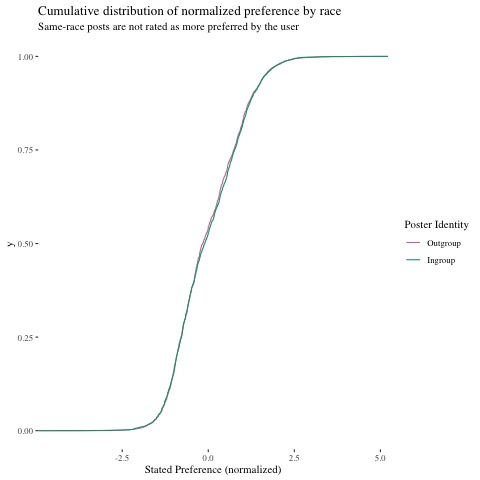
\includegraphics[scale=.8]{Output/Graphs/Audit/Stated preferences/US NF cdf norm preferences by ingroup.jpg}
    \caption{CDF}
    \label{fig:prefcdf}
\end{figure}

%%%%%% Prolific Survey Appendix %%%%%% 
\section{Prolific Survey Details}\label{app:survey}

Details on data collection, sample recruitment, and questions for automaticity survey

%%%%%% India Appendix %%%%%% 
\section{India Data Collection}\label{app:india}
Some details about the India Data Collection

\subsection{Tables and Figures for India Data}

%%%% NF %%%%
\begin{figure}[ht]
\caption{NF in-group Posts Higher}
\label{fig:nf_bygroup_india}
    \begin{subfigure}{.5\textwidth} 
        \centering
        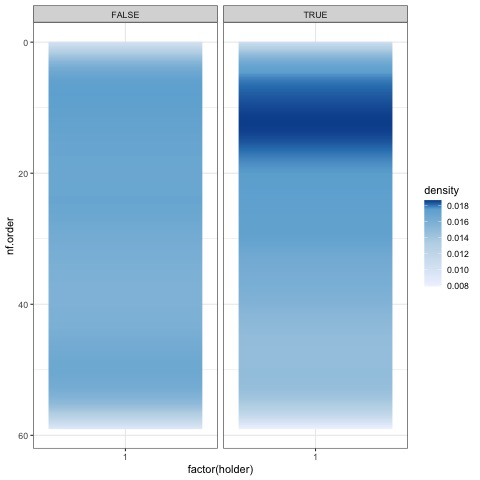
\includegraphics[width=1\linewidth]{Output/Graphs/Audit/Heatmaps/India NF nf rank by ingroup - smooth.jpg}  
        \caption{Two Single Heat Maps by in-group}
        \label{fig:nf_bygroup_hm}
        \end{subfigure}
    \begin{subfigure}{.5\textwidth}
        \centering
        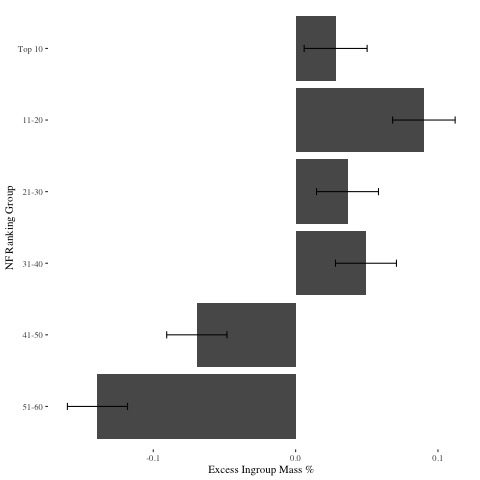
\includegraphics[width=.9\linewidth]{Output/Graphs/Audit/Excess Mass/India NF excess mass by ranking group.jpg}  
        \caption{Excess Mass by Ranking}
        \label{fig:nf_bygroup_em_india}
    \end{subfigure}
\end{figure}

\begin{figure}[ht]
\caption{NF Beautiful Results}
\label{fig:nf_main_india}
    \begin{subfigure}{.5\textwidth} 
        \centering
            % include first image
        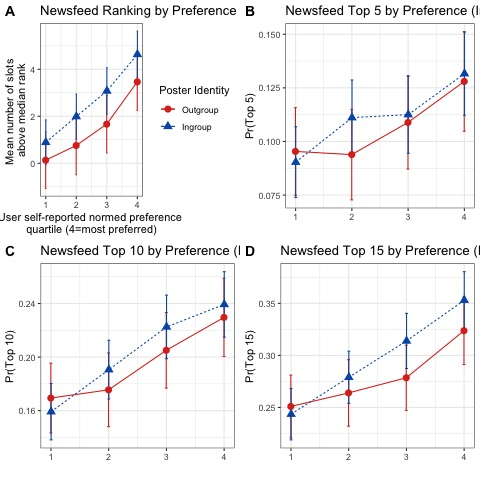
\includegraphics[width=1\linewidth]{Output/Graphs/Audit/Ranking line graphs/India NF all outcomes panel by norm preference by ingroup.jpg} 
        \caption{Something1}
        \label{fig:nf_line_india}
        \end{subfigure}
    \begin{subfigure}{.5\textwidth}
        \centering
        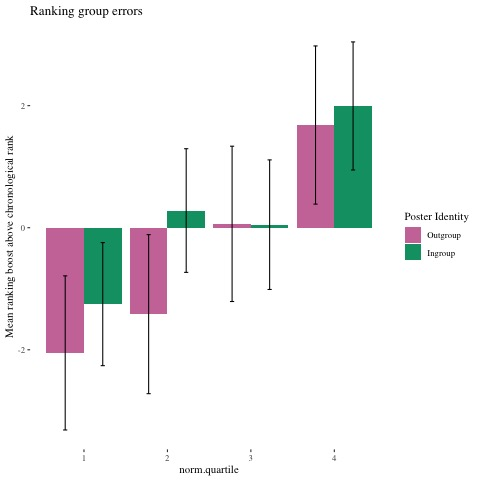
\includegraphics[width=1\linewidth]{Output/Graphs/Audit/Misranking relative to expectation/Chronological expectation/India NF by norm preference.jpg}  
        \caption{Something2}
        \label{fig:nf_rankingboost_india}
    \end{subfigure}
\end{figure}

%%%% PYMK %%%%
\begin{figure}[ht]
\caption{PYMK in-group Posts Not Higher}
\label{fig:pymk_bygroup_india}
    \begin{subfigure}{.5\textwidth} 
        \centering
        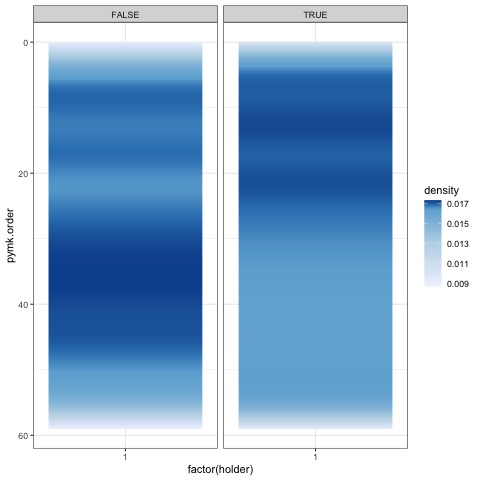
\includegraphics[width=1\linewidth]{Output/Graphs/Audit/Heatmaps/India PYMK pymk rank by ingroup - smooth.jpg}  
        \caption{Two Single Heat Maps by in-group}
        \label{fig:pymk_bygroup_hm_india}
        \end{subfigure}
    \begin{subfigure}{.5\textwidth}
        \centering
        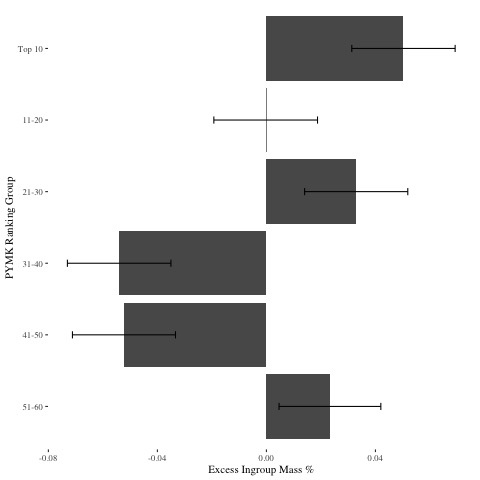
\includegraphics[width=.9\linewidth]{Output/Graphs/Audit/Excess Mass/India PYMK excess mass by ranking group.jpg}  
        \caption{Excess Mass by Ranking PUT ON SAME SCALE AS NF?}
        \label{fig:pymk_bygroup_em_india}
    \end{subfigure}

\end{figure}

\begin{figure}[ht]
\caption{PYMK Results}
\label{fig:pymk_main_india}
    \begin{subfigure}{.5\textwidth} 
        \centering
            % include first image
        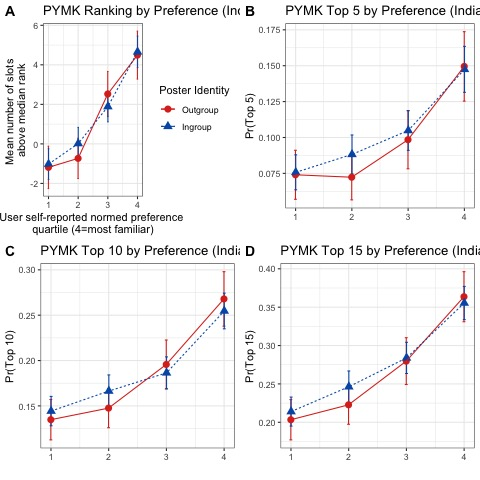
\includegraphics[width=1\linewidth]{Output/Graphs/Audit/Ranking line graphs/India PYMK all outcomes panel by norm preference by ingroup.jpg} 
        \caption{Something1}
        \label{fig:pymk_line_india}
        \end{subfigure}
    \begin{subfigure}{.5\textwidth}
        \centering
        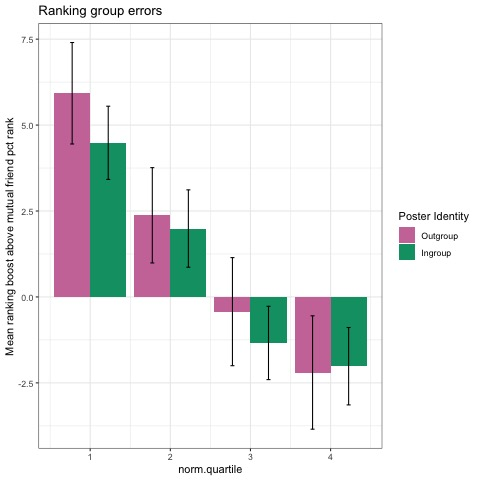
\includegraphics[width=1\linewidth]{Output/Graphs/Audit/Misranking relative to expectation/Mutual friends expectation/India PYMK by norm pref.jpg}  
        \caption{Something2}
        \label{fig:pymk_rankingboost_india}
    \end{subfigure}

\end{figure}

\begin{table}[!htbp] \centering 
  \caption{Experiment 1} 
  \label{} 
\begin{tabular}{@{\extracolsep{5pt}}lcc} 
\\[-1.8ex]\hline 
\hline \\[-1.8ex] 
 & \multicolumn{2}{c}{\textit{Dependent variable:}} \\ 
\cline{2-3} 
\\[-1.8ex] & human choice & algorithm rank \\ 
\\[-1.8ex] & (1) & (2)\\ 
\hline \\[-1.8ex] 
 In-group & 0.031$^{***}$ & $-$2.099$^{***}$ \\ 
  & (0.007) & (0.304) \\ 
  & & \\ 
 More deliberation & 0.014 & $-$0.768$^{**}$ \\ 
  & (0.009) & (0.367) \\ 
  & & \\ 
 In-group x Deliberation & $-$0.017$^{*}$ & 1.053$^{**}$ \\ 
  & (0.010) & (0.430) \\ 
  & & \\ 
 Constant & 0.164$^{***}$ & 14.951$^{***}$ \\ 
  & (0.006) & (0.260) \\ 
  & & \\ 
\hline \\[-1.8ex] 
Observations & 26,094 & 11,886 \\ 
R$^{2}$ & 0.001 & 0.005 \\ 
Adjusted R$^{2}$ & 0.001 & 0.005 \\ 
\hline 
\hline \\[-1.8ex] 
\textit{Note:}  & \multicolumn{2}{r}{$^{*}$p$<$0.1; $^{**}$p$<$0.05; $^{***}$p$<$0.01} \\ 
\end{tabular} 
\end{table} 

\begin{table}[!htbp] \centering 
  \caption{Experiment 2} 
  \label{} 
\begin{tabular}{@{\extracolsep{5pt}}lcc} 
\\[-1.8ex]\hline 
\hline \\[-1.8ex] 
 & \multicolumn{2}{c}{\textit{Dependent variable:}} \\ 
\cline{2-3} 
\\[-1.8ex] & human choice & algorithm rank \\ 
\\[-1.8ex] & (1) & (2)\\ 
\hline \\[-1.8ex] 
 In-group & 0.005 & $-$3.326$^{***}$ \\ 
  & (0.009) & (0.410) \\ 
  & & \\ 
 More deliberation & $-$0.003 & $-$1.197$^{**}$ \\ 
  & (0.011) & (0.534) \\ 
  & & \\ 
 In-group x Deliberation & 0.003 & 1.413$^{**}$ \\ 
  & (0.012) & (0.580) \\ 
  & & \\ 
 Constant & 0.127$^{***}$ & 17.998$^{***}$ \\ 
  & (0.008) & (0.378) \\ 
  & & \\ 
\hline \\[-1.8ex] 
Observations & 22,833 & 10482 \\ 
R$^{2}$ & 0.0001 & 0.008 \\ 
Adjusted R$^{2}$ & $-$0.0001 & 0.008 \\ 
\hline 
\hline \\[-1.8ex] 
\textit{Note:}  & \multicolumn{2}{r}{$^{*}$p$<$0.1; $^{**}$p$<$0.05; $^{***}$p$<$0.01} \\ 
\end{tabular} 
\end{table} 

\begin{center}
\begin{tabular}{||l c c||} 
 \hline
 Variable & Experiment 1 & Experiment 2\\ [0.5ex] 
 \hline\hline
Number of participants & 981 & 753\\ 
 \hline
 Number of selected movies & 4,859 & 3,001 \\
 \hline
 Male & 0.39 & 1.00 \\
 \hline
 Mean age & 29.6 & 38.8 \\  
 \hline

 Race &  &  \\
 \hline
 \hspace{1cm} Black & 0.14 & 0.00 \\
 \hline
 \hspace{1cm} Hispanic & 0.23 & 0.00 \\
 \hline
 \hspace{1cm} White & 0.63 & 1.00 \\
 \hline
 \hspace{1cm} Other & 0.01 & 0.00 \\
 \hline
 Education &  &  \\
 \hline
 \hspace{1cm} Less than bachelor's & 0.37 & 0.44 \\
 \hline
 \hspace{1cm} Bachelor's & 0.32 & 0.37 \\
 \hline
 \hspace{1cm} More than bachelor's & 0.31 & 0.19 \\
 \hline
\end{tabular}
\end{center}

\end{document}
